\documentclass[12pt,a4paper,boxed,titlepage]{caspset}

% set 1-inch margins in the document
%\usepackage[left=1in,right=1in,top=1.2in,bottom=1in]{geometry}
\usepackage[left=1in,right=1in,top=1.2in,bottom=1in]{geometry}
\usepackage{lastpage}
\usepackage{multicol}
% include this if you want to import graphics files with /includegraphics
\usepackage{graphicx}
\usepackage{lscape}
\usepackage{amsmath,amsfonts,amsthm,amssymb}
\usepackage{hyperref}
\usepackage{setspace}
\usepackage{fancyhdr}
\usepackage{lastpage}
\usepackage{extramarks}
\usepackage{chngpage}
\usepackage{soul}
\usepackage[usenames,dvipsnames]{color}
\usepackage{graphicx,float,wrapfig}
\usepackage{ifthen}
\usepackage{listings}
\usepackage{courier}
\usepackage{multimedia}
\usepackage[toc,page,title,titletoc,header]{appendix}
\usepackage{color, soul}
\usepackage{tikz}
\usepackage{array}
\usepackage{multirow}
\usepackage{todonotes}
\usepackage{pdfpages}
\usetikzlibrary{%
    decorations.pathreplacing,%
    decorations.pathmorphing,arrows
}
%%%%%%%%%%%%%%%%%%%%%%%%%%%%%%%%%%%%%%%%%%%%%%%%%%%%%%
\usepackage{xeCJK}
%\usepackage{fontspec}
\setCJKmainfont[BoldFont=simhei.ttf]{simsun.ttf}
\setCJKsansfont{simhei.ttf}
\setCJKmonofont{simfang.ttf}

%\setCJKmainfont{Adobe Song Std}
%\setCJKmainfont[BoldFont=Adobe Heiti Std]{Adobe Song Std}
%%%%%%%%%%%%%%%%%%%%%%%%%%%%%%%%%%%%%%%%%%%%%%%%%%%%%%

\graphicspath{{figures/}}

\setulcolor{red}

\setlength{\marginparwidth}{1in}

\newcommand{\hmwkTitle}{力学实验与技术原理}
\newcommand{\hmwkSubTitle}{} % No subtitle, so this will be excluded
\newcommand{\hmwkDueDate}{\today}
\newcommand{\hmwkClass}{物理学院}
\newcommand{\hmwkClassTime}{}
\newcommand{\hmwkClassInstructor}{李战华等}
\newcommand{\hmwkAuthorName}{周吕文}


\hypersetup{pdfauthor={\hmwkAuthorName}, 
            pdftitle={超声速流声显示实验}, 
            pdfsubject={\hmwkTitle, \hmwkClassInstructor},
            pdfkeywords={力学实验, 实验报告},
            pdfproducer={XeLateX with hyperref},
            pdfcreator={Xelatex}}


%% Setup the header and footer
\pagestyle{fancy}                                                       %
\lhead{\hmwkAuthorName}                                                 %
\chead{\hmwkClass\ (\hmwkClassInstructor\ \hmwkClassTime): \hmwkTitle}  %
\rhead{第\ \thepage\ 页, 共\ \protect\pageref{LastPage} 页}          %



\makeatletter
\newcommand{\rmnum}[1]{\romannumeral #1}
\newcommand{\Rmnum}[1]{\expandafter\@slowromancap\romannumeral #1@}
\makeatother

\renewcommand\refname{\bf\large 参考文献}
\renewcommand\contentsname{\bf 目 \ \ \ 录}
\renewcommand\figurename{\bf 图}
\renewcommand\tablename{\bf 表}
\renewcommand\appendixname{\bf 附录}
\renewcommand{\appendixpagename}{附录}
\renewcommand\listfigurename{图目录}

% info for header block in upper right hand corner
%\name{周吕文{~}201128000718065}
%\class{物理学院{~}20110308班}
%\assignment{习题整理}
%\duedate{06/14/2014}


\begin{document}

\includepdf{cover}
\setlength{\parskip}{0.3em}
\setcounter{page}{0}
\tableofcontents
\listoffigures

\newpage
\section{实验背景}

在现代科学技术的研究中, 实验技术是最活跃的领域之一. 现代科学技术研究的关键问题在于根据实验结果进行研究分析并建立研究对象的物理模型, 而不是根据猜测. 流体力学研究中的流场显示技术, 其任务就是把存在于透明介质空气、水等中的流动现象(其中很多现象是直接看不见的)设法用图像显示出来, 并力求做到根据这些图像作流场某些物理量的定量测定.

\begin{multicols}{2}
流场显示实验可以追溯到1883年雷诺的流场显示实验(左图即为雷诺和他的实验装置)发表, 在这一百多年里, 流场显示实验在科学发展上起了很大的作用. 以气动力学为例, 一旦被研究的流动图案(流谱)被显示出来以后, 问题往往较快地被解决, 无论在理论研究和实验研究上都起了很大的推动作用. 例如湍流、涡流、边界层等现象都是首先被流场显示实验观察到的. 随着流体力学的发展, 流场显示技术也不断地得到发展. 自雷诺的流场显示实验后, 这门技术的原理性和技术性文献不断涌现, 形成了一门独特的实验技术科学, 到前为止, 仍然显示它的活跃和生命力. 它的发展总是和科学发展、新技术的发展相联系的, 例如激光的出现促进了全息术的迅猛发展, 而全息照相和全息干涉术又为流场显示领域增添革命性的内容和发展, 例如为解决三维流场的定量测量开拓了道路.

\begin{center}
\fbox{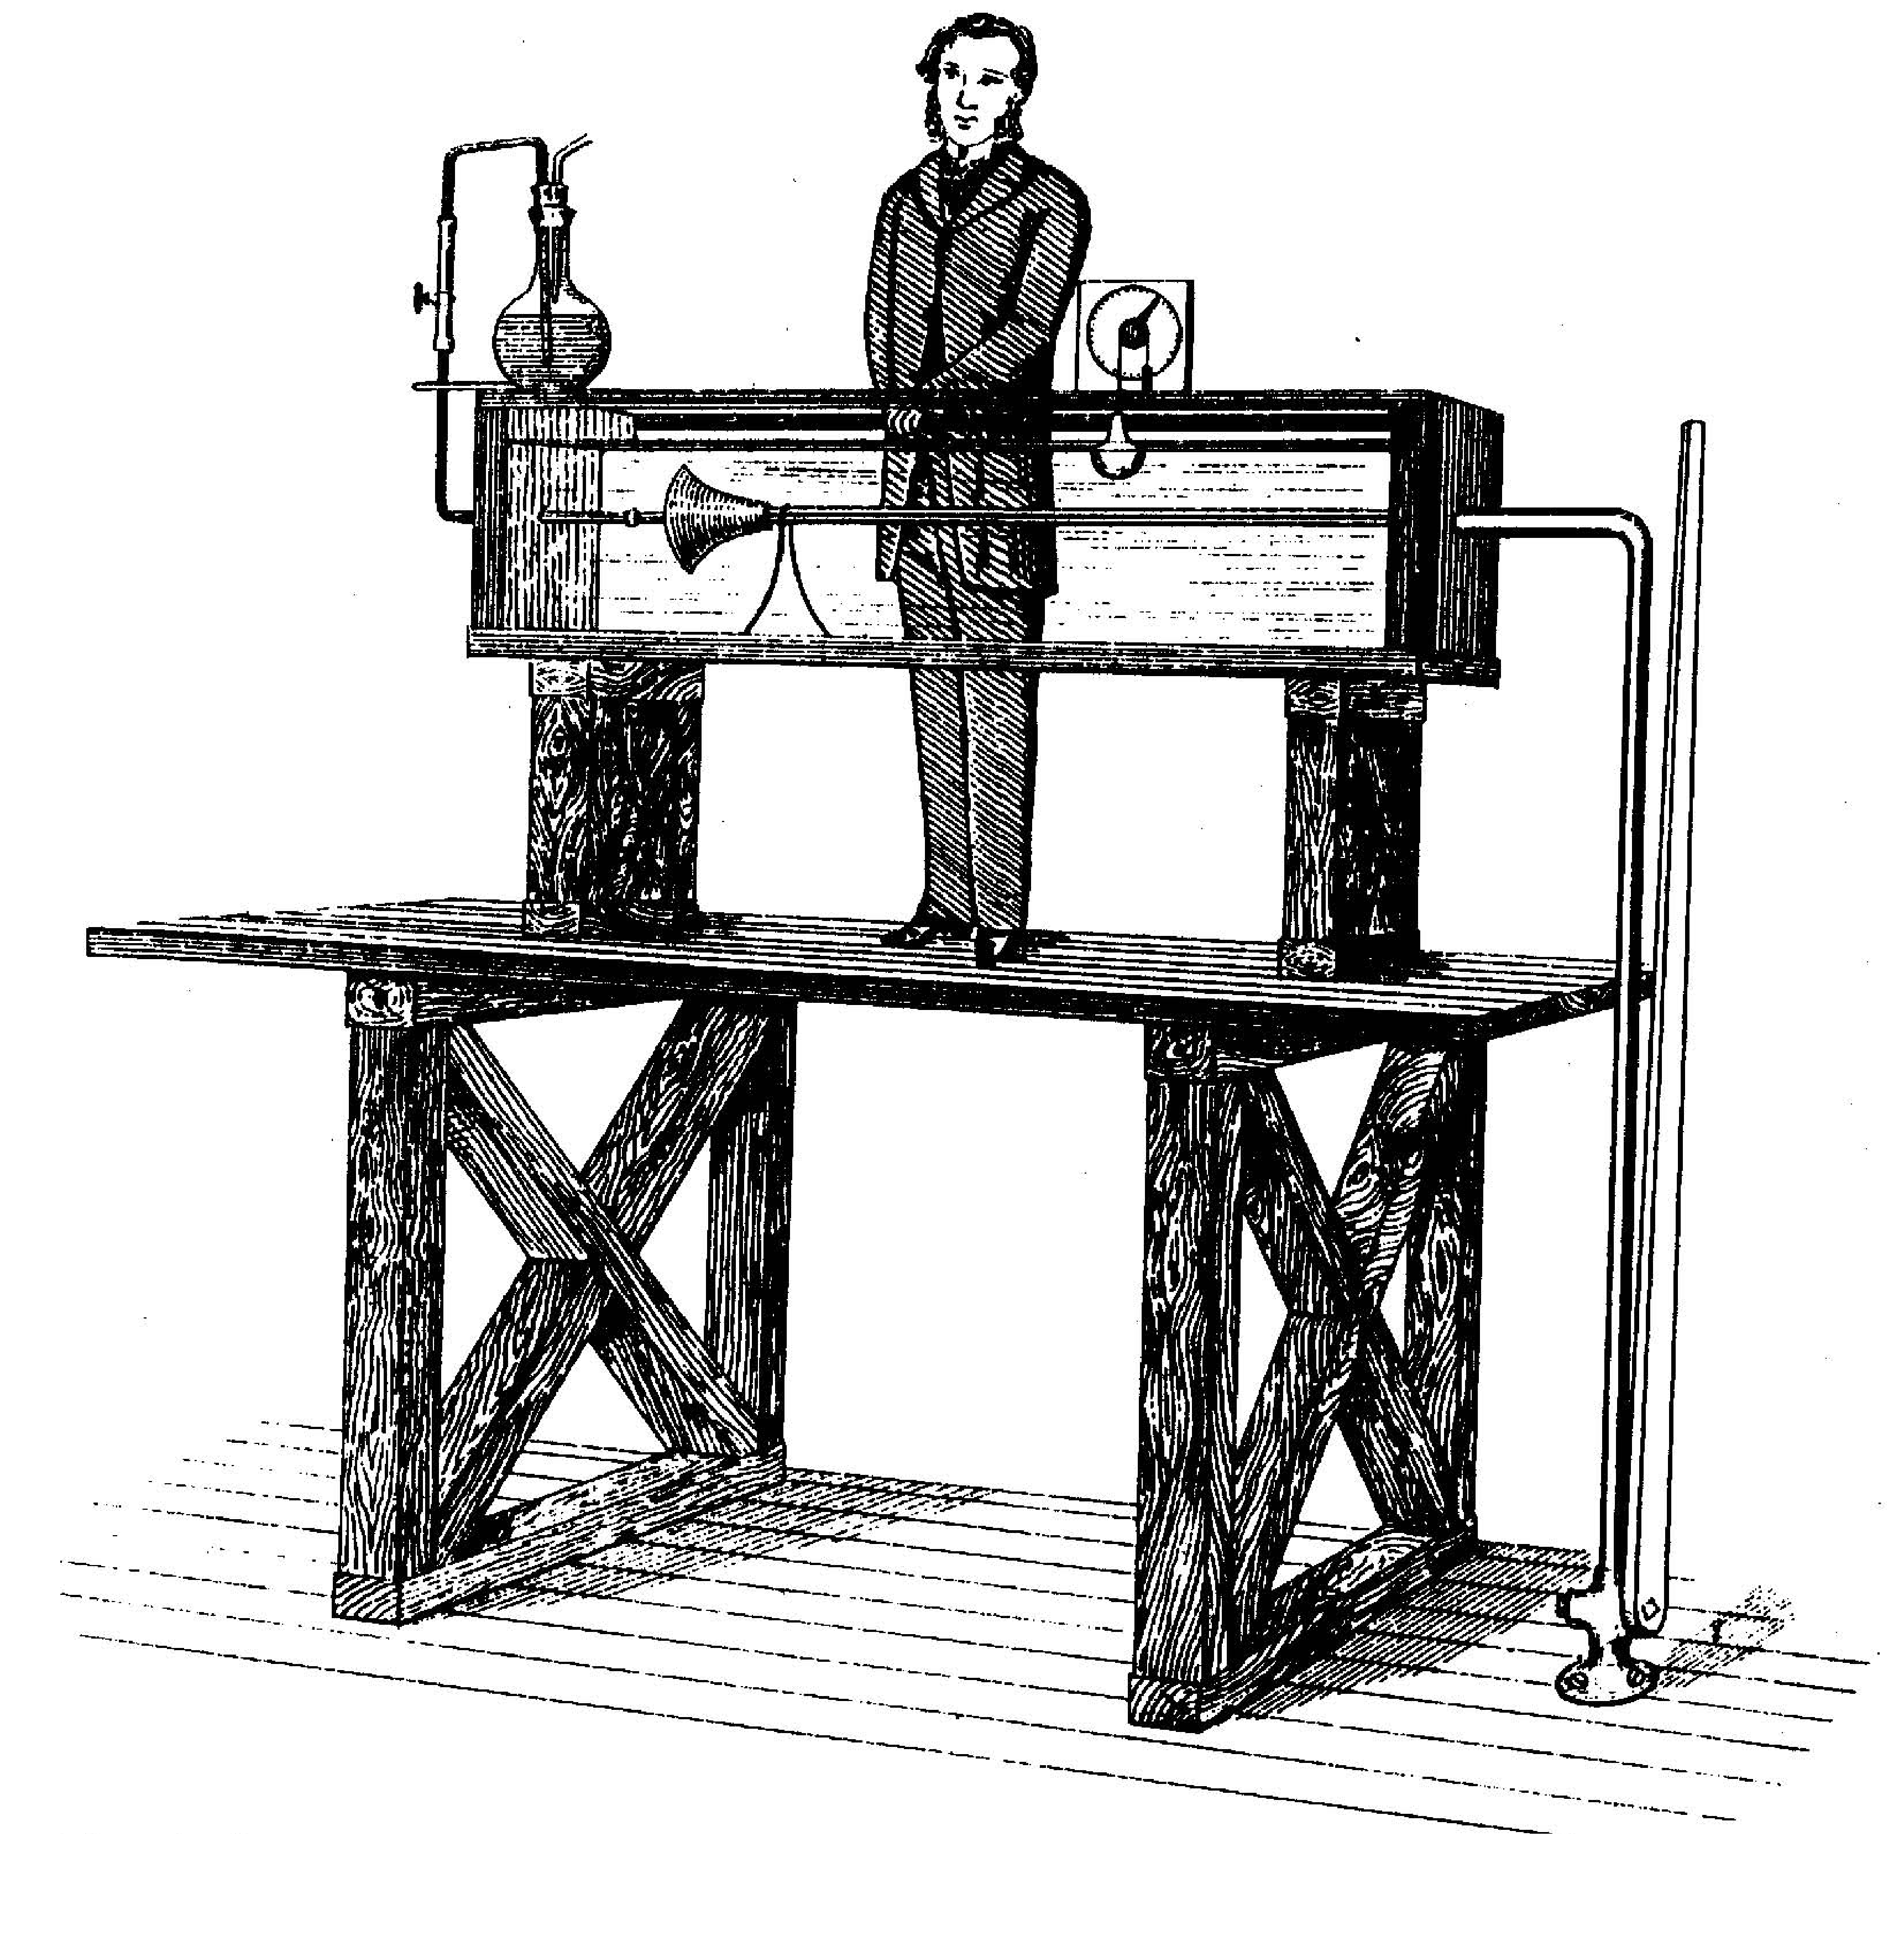
\includegraphics[width=0.425\textwidth]{Reynold.pdf}}
\end{center}

\end{multicols}

流场显示技术目前已被广泛应用于流体力学、空气动力学、爆炸力学、等离子体物理、燃烧学、传热学、核子物理、大气物理、空间技术和化学反应工程等一系列领域中。特别是在风洞实验中, 流场显示是确定流谱等物理现象可靠而有效的方法。电子计算机的发展, 并没有降低流场显示的作用, 因为只有更精确的物理模型才能使流休力学有所发展, 而空气动力学中的理论还远未完善, 还需要流场显示继续提供数据。

现代流场显示技术, 不仅可以提供由于压力变化、温度变化、密度变化速度变化和离子浓度变化等物理量变化所描述的图案, 并且有些方法还可提供定量的测量数据. 在数据的采集方式上, 具有速度快、不扰动流动场、空间大信息量采集的能力等优点, 是其他测量技术难以做到的。

现代流场显示流场显示技术可分为两大类: 在流场中掺入外来物质或注入能量的显示方法和光学显示测量方法. 在流场中掺入外来物质或注入能量的显示方法通过往流场中掺入颜料,气泡等或引入火花,热质点,电子束等显示流场的行为。光学显示测量方法主要是利用阴影照相技术、纹影照相技术、干涉技术、全息照相、全自、干涉以及付氏光学信息处理技术等技术来显示流场的行为。本文的实验就属于光学显示测量方法,利用阴影照相技术和纹影照相技术对流场进行显示。

\section{实验目的}
超声速流动的研究对远程导弹和人造卫星等超声速飞行器的研制具有重要指导意义。因此,超声速流场显示是非常必要也是非常重要的。
超声速流场显示实验即激波与膨胀波的阴影和纹影显示实验, 实验目的主要有:
\begin{itemize}
\item 了解纹影法和阴影法测流场的光学原理.
\item 撑握纹影法和阴影法测流场实验光路的搭建和调试方法.
\item 了解纹影法和阴影法对同一流场测试结果的差异.
\end{itemize}

\section{实验设备}

实验设备主要有CCD高速摄相机, 光学仪器组(包括激光发生器, 凸透镜, 凹面镜等), 超燃风洞, 尖劈等. 下面重点介绍以下设备:
\begin{itemize}
\item \textbf{高速摄相机CCD}

高速摄像机就是能够以很高的频率记录一个动态的图像, 因为一个动态的图像是需要数个静止的连贯的图片按一定时间速度播放出来的, 高速摄像机一般可以每秒1000-10000帧的速度记录, 但这导致了每张像素不会太高, 另外它也要有一个惊人的储存器.
本次实验室要观察激波与膨胀波的纹影, 阴影显示的动态变化过程, 照相时频率为5000帧/秒.

\item \textbf{光学仪器组}

\textbf{光源}:在阴影系统中, 为了得到清晰的阴影像, 必须用有一定亮度的点光源. 在纹影系统中, 光源的尺寸, 形状及其亮度是重要的参数, 影响纹影系统的敏感度和偏折范围, 而且光源亮度又是影响曝光时间的重要因素. 对于脉冲闪光光源而言, 闪光的短持续时间对于不稳定流动现象的纹影流场显示记录是十分重要的. 由于激光的单色性好, 较高的脉冲频率和极短的闪光持续时间, 直线性和亮度大等特点, 对于光学流场显示和高速照相有特别的意义. 本次实验用的是氩灯冷光源, 其输入功率470VA.

\textbf{凹面镜}: 焦距1470mm, 曲率半径3010mm, 半径147mm.

\item \textbf{超燃风洞:}马赫数$M=2.5$.
\end{itemize}

\section{实验原理}
本节中, 在\ref{basic}先说明光学显示测量方法(主要是阴影法和纹影法)基本光学原理, 在 \ref{basicshadow} 和 \ref{basicschlieren}分别详细说明阴影法和纹影法的原理, 最后在\ref{diff}谈谈两种方法在原理上的差异.

\subsection{基本光学原理}\label{basic}
光在不同介质中的传播速度是不同的, 与介质的折射率$n$有关. 用光学方法进行高速流场显示的物理基础就是基于上述的折射现象. 对于某一特定气体, 其绝对折射率定义为:
\[
n = \frac{c}{v} = 1 + \frac{c-v}{v} = 1 + \frac{\Delta\lambda}{\lambda}
\]
其中$c$为光在真空中的传播速度; $v$为光在介质中的传播速度; $\lambda$为光在该气体中传播的波长;  $\Delta\lambda$为光在气体介质中和真空中波长的变化. 对于一定的介质, 其折射率是介质密度的函数, 当n接近为1时, 通常可以将上式近似表达为
\[
\frac{n-1}{\rho} = K_{GD} {~}\textrm{或}{~} n=1+K_{GD}\rho
\]
上式称为Gladstone-Dale公式, 其中$K_{GD}$为常数, 是气体的一种特性, 称为比折射度. 一般情况下, 气体密度$\rho$与气体折射率$n$的关系可用上述Gladstone-Dale公式表示.

因此, 在一个密度不均匀的介质中, 如在有密度变化的流场中, 各个部分的折射率是不同的.流场气体密度的变化会引起气体的光学折射率变化, 从而改变光束传输的路径, 光束偏离原来的方向, 形成一个偏折角, 被扰动的光束发生相位变化.
\begin{figure}[!htb]
\centering
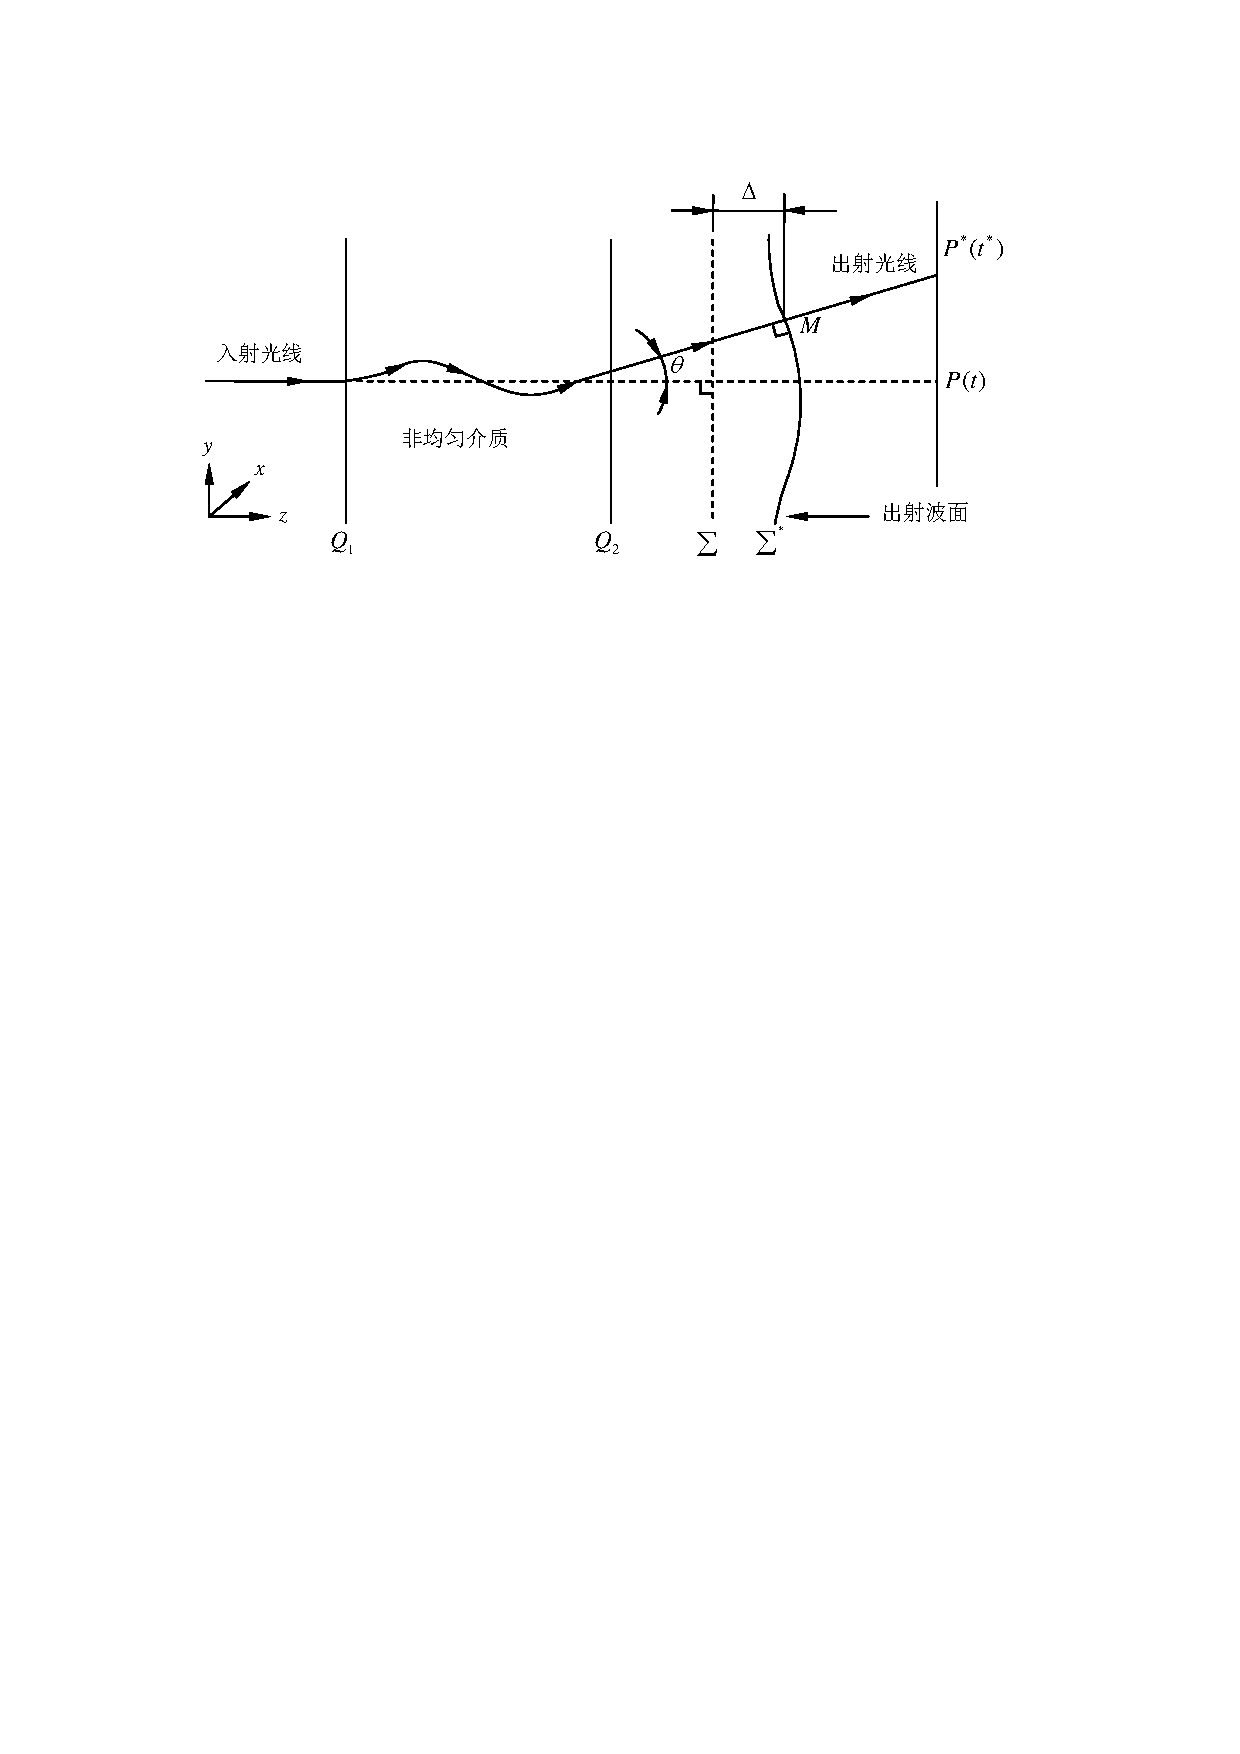
\includegraphics[width=0.7\textwidth]{optics.pdf}
\caption{\label{optics}光线传输过程中的三个变量}
\end{figure}
例如图\ref{optics}中, 在扰动区中被偏折的光线到达投影屏上的$p^*$点, 而不是无扰动时的$P$点, 因此投影屏上的光强分布相对于未扰动时的光强分布发生了变化. 在$p^*$ 点位置接收的光量比原来更多, 投影屏上显示的是光强分布的相对值, 所以呈现为明暗相间的阴影条纹, 阴影亮度的变化体现了光束偏折的方向和大小的变化. 在图\ref{optics}的光线传输过程中, 存在三个变量:
\begin{enumerate}
\item 接收屏上的位移量($P^*P$).
\item 扰动光线相对于未扰动光线的角偏移($\theta^*-\theta$).
\item 由光线的光程差引起的相位变化($\varphi^*-\varphi$).
\end{enumerate}
所有显示流畅的光学方法的基础是记录光线被扰动后的偏折位移, 偏折角和相位差, 三者分别对应的是密度的二阶导数, 一阶导数和密度的变化.

\subsection{阴影法}\label{basicshadow}
这方法一般认为是V.Dvorak于1880年创立的. 它所需设备简单, 易于实现, 然而效果良好. 现代阴影技术使用短的光脉冲光源得到非常清晰的阴影图, 可显示紊流区中的流动, 尾迹流中的旋涡, 边界层中的转挨情况等流动细节. 阴影图表征流场密度梯度的梯度($\partial^2\rho/\partial x^2$)图像直观, 因而目前仍被广泛应用. 图\ref{shadow01}所示阴影仪的光路布置图.
\begin{figure}[!htb]
\begin{minipage}[b]{.5\textwidth}
\centering
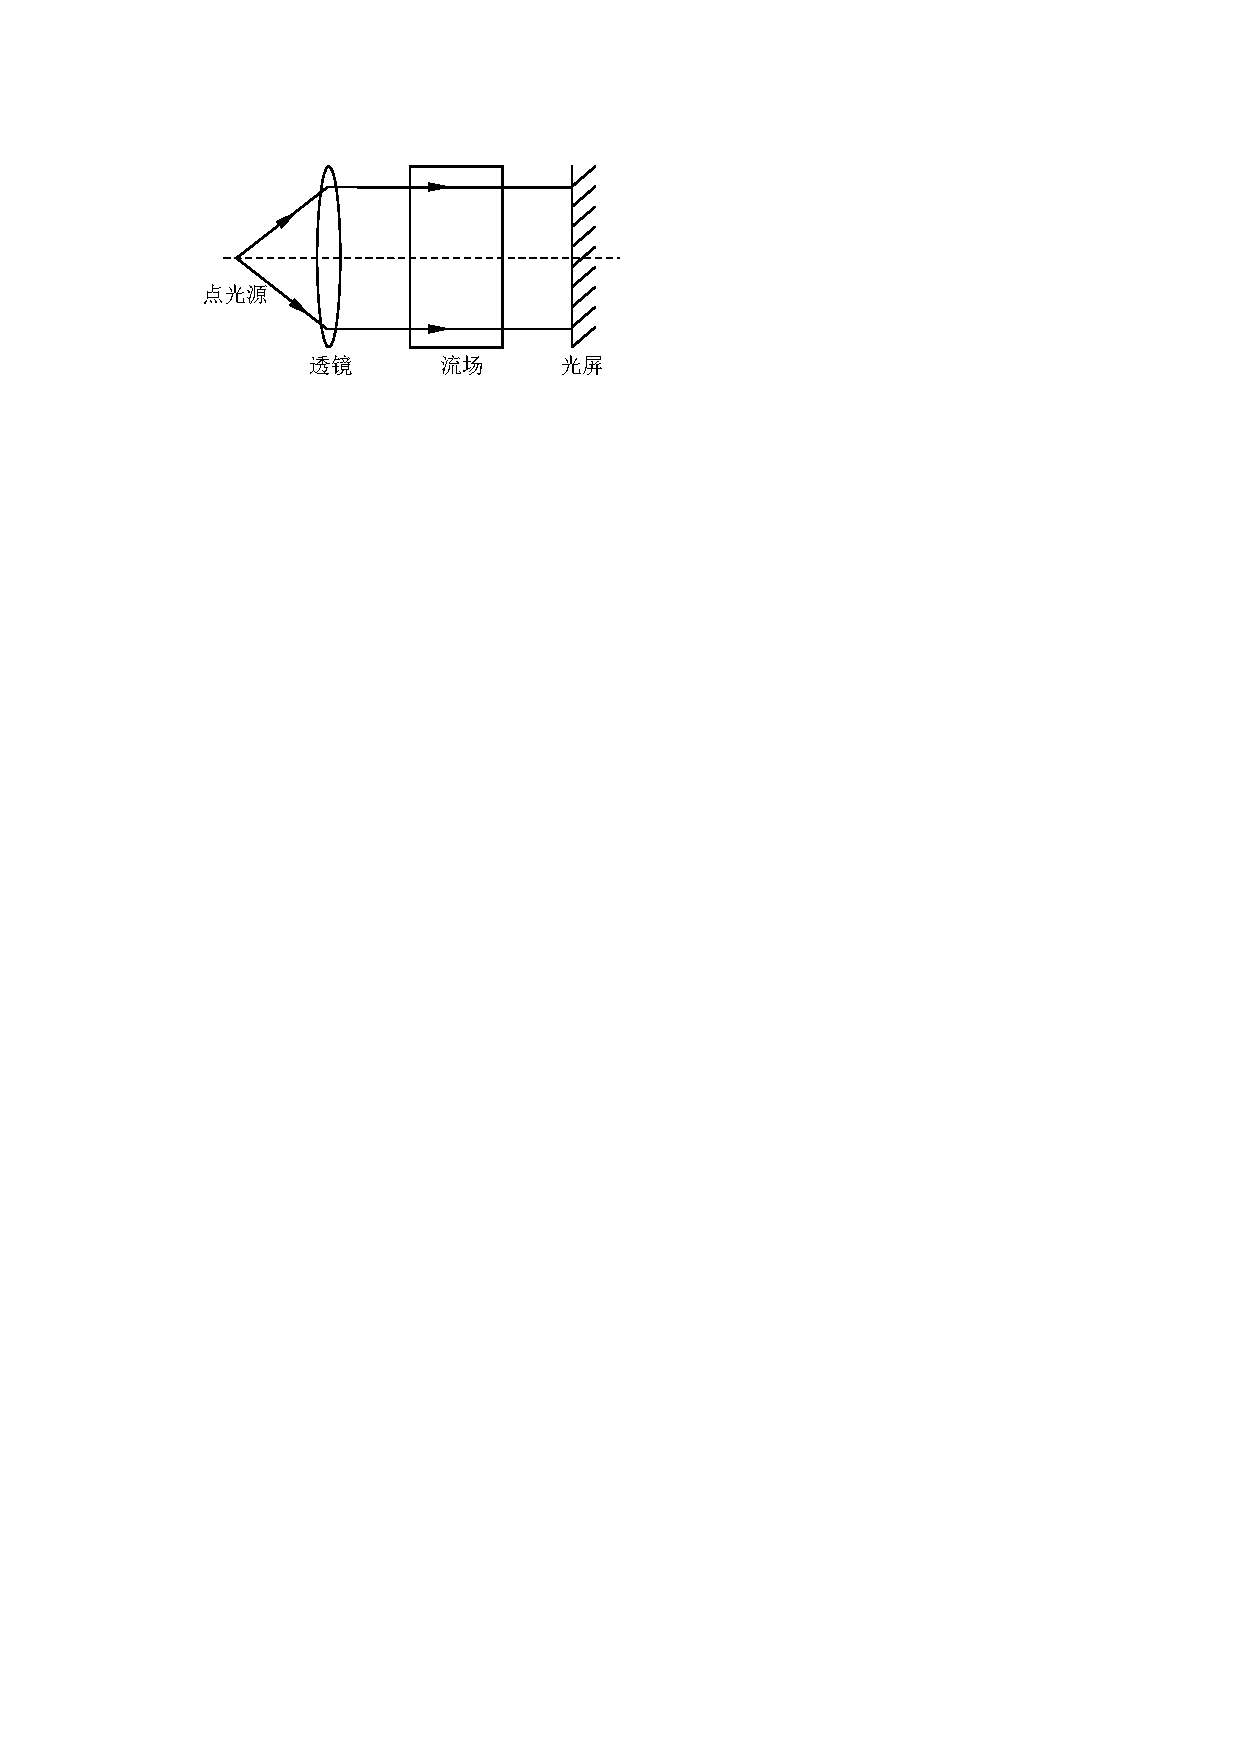
\includegraphics[width=0.7\textwidth]{shadow01.pdf}
\caption{\label{shadow01}阴影法原理图}
\end{minipage}%
\begin{minipage}[b]{.5\textwidth}
\centering
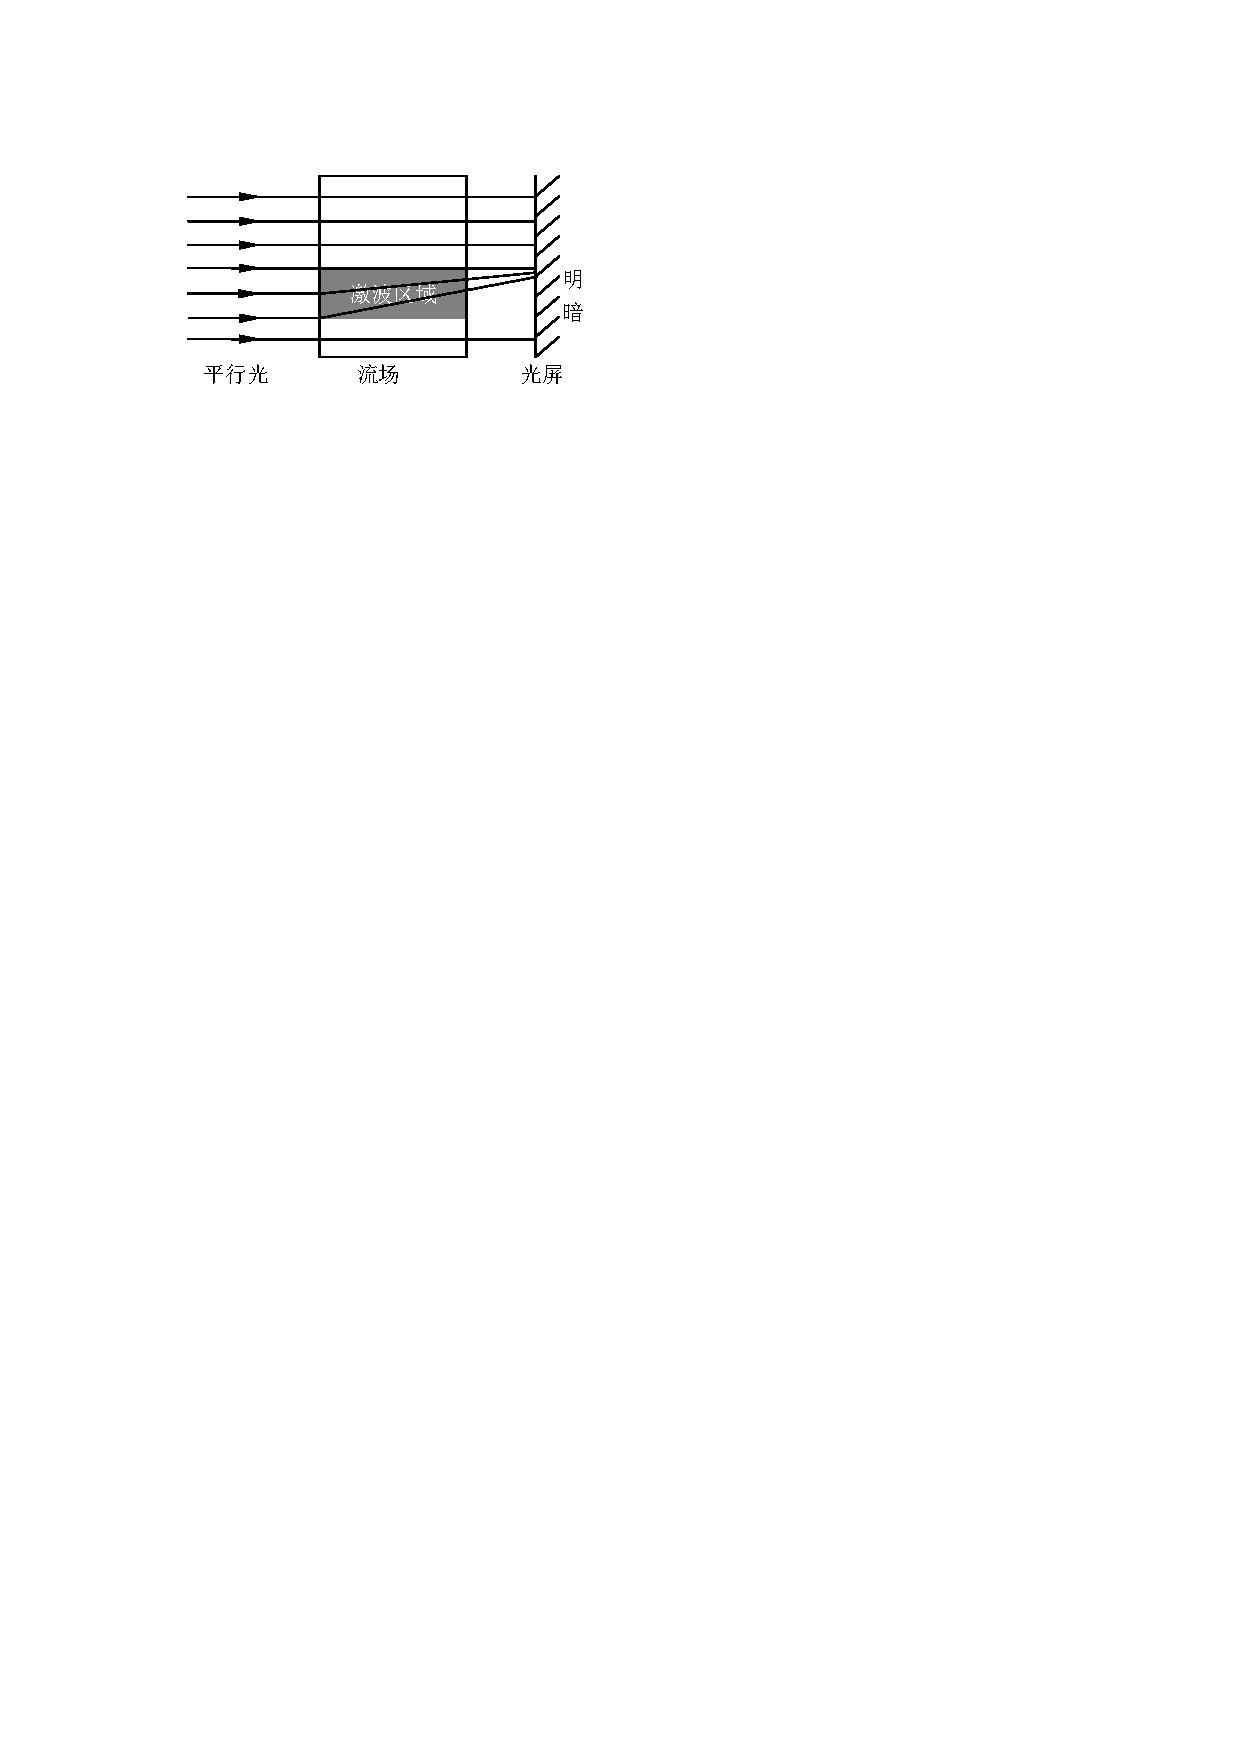
\includegraphics[width=0.7\textwidth]{shadow02.pdf}
\caption{\label{shadow02}激波阴影示意图}
\end{minipage}
\end{figure}

阴影法的原理, 可用图\ref{shadow01}说明. 点光源置于试验段一侧, 经过透镜成为平行光束, 通过试验段再投射到屏幕上, 风洞启动前流场密度均匀分布, 屏幕上显示均匀的亮度. 风洞启动后, 实验段内由于放置模型, 流场收到扰动, 模型周围成为光路中的扰折区. 在扰折区内, 各点的密度不再是均匀分布的, 各点的折射率也各不相同. 射入这一区域的光线将由其入射方向偏折, 因而屏幕被扰折区光线投射的位置, 将出现明暗不均的情况. 流场中密度变化越是明显, 屏幕上对比越是强烈.

图\ref{shadow02}是激波阴影形成的原理. 如果流场中各点的折射率相同. 即折射率的二阶导数等于0, 则原来的平行光束透过流场偏折了同样的角度. 因而光线依然保持平行. 于是屏幕上光线的亮度依然保持均匀不变.
由于激波区存在很大的密度梯度, 其折射率变化十分剧烈. 在激波前锋部分, 折射率的变化率, 即折射率的二阶导数$\partial^2n/\partial x^2>0$, 光线散开, 因此这部分在屏幕上很暗. 而激波的后半部, $\partial^2n/\partial x^2<0$, 这时光线聚拢, 于是屏幕上相应部分被照亮.
因此, 屏幕上的亮度是$\partial^2\rho/\partial x^2$的函数. 这些明暗区的出现是由于折射偏折 $\Delta s$的变化导致的. 照度的变化粗略的正比与折射率的二阶导数.

\subsection{纹影法}\label{basicschlieren}

纹影法的原理与阴影法一样都是基于光的折射. 纹影图表示流场密度梯度的变化, 灵敏度比阴影法高一个量级, 可以用来较为细致稳定的显示高速流场.
纹影法是在阴影法光路的基础上增加纹影透镜和刀口光阑装置而实现的,如图\ref{schlieren01}, 纹影图表征流场密度梯度 ($\partial\rho/\partial x$).
\begin{figure}[!htb]
\centering
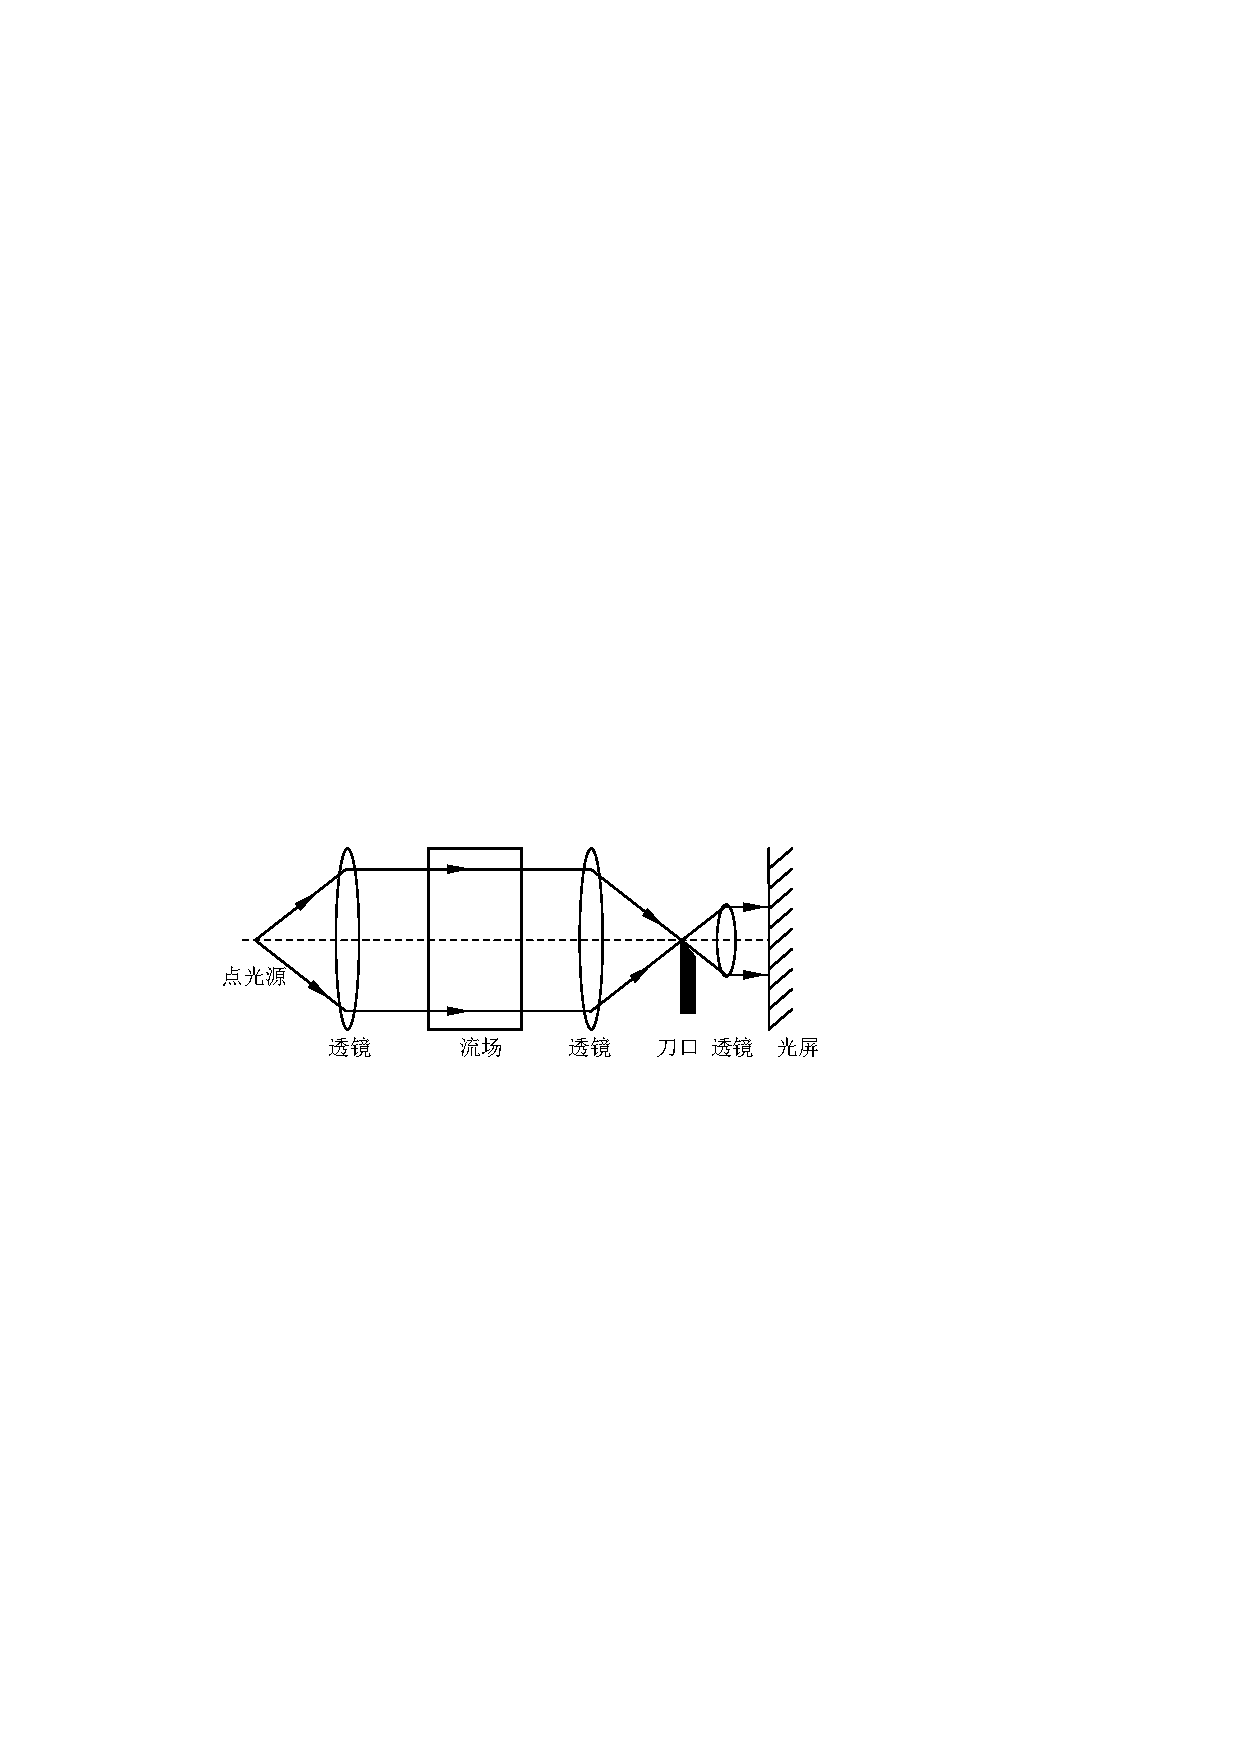
\includegraphics[width=0.6\textwidth]{schlieren01.pdf}
\caption{\label{schlieren01}纹影法原理图}
\end{figure}

平行光束穿过流场, 经过纹影透镜使线光源成像于纹影透镜的焦平面上. 在焦平面上安置可上下左右调节的刀口光阑, 即``光刀''. 光阑后面再用一投影物镜将物象投影到屏幕上. 刀口光阑的作用是切割光线, 它可把线光源射来的光线挡去一部分, 使屏幕上亮度减弱.

风洞启动前, 实验段内流场是均匀的. 启动后, 流场中气流不均匀, 密度发生了变化(如流场中存在激波), 则某一些光线就会发生偏折. 向上折射$\Delta\theta$角的光线就会越过刀口光阑射到屏幕上, 幕上某些点由于额外多照射一些光线, 就比其他点亮一些. 同理, 向下折射$\Delta\theta$的这部分光线就受到刀口光阑的阻挡, 幕上某些点就会比原来暗一些. 这样, 屏幕上的亮度变化就反应了流场中密度的变化.

由此可见, 屏幕上各点的阴暗程度完全取决于光线的偏折角$\Delta\theta$, 也可以直接取决于流场中光线的折射率梯度$\partial n/\partial x$, $\partial n/\partial y$或者气流密度$\partial\rho/\partial x$, $\partial
\rho/\partial y$. 折射率阶导数产生的照度变化就是纹影. 由于纹影法比阴影法灵敏的多, 又由于刀口光阑位置可以调节, 事先可让屏幕阴暗一些, 光线折射后引起的明暗差别更为显著, 这样可以分辨流场中密度很小的变化.

\subsection{阴影法和纹影法的差异}\label{diff}

在阴影法和纹影法测流场的实验中, 光强的变化$\Delta I/I$与密度$\rho$的关系式为:
\[
\frac{\Delta I}{I} \approx
l \cdot
\int_\zeta^{\zeta_1}
\frac{K_{GD}}{n}\Big(
\frac{\partial^2\rho}{\partial x^2} + \frac{\partial^2\rho}{\partial y^2}
\Big)
\]
由此可见, 阴影法对密度的二阶导数变化量敏感, 由于做了近似处理, 存在较大误差, 阴影法只能用作定性分析.

阴影法只对密度的二阶导数灵敏, 适用于密度梯度变化显著的流场显示, 如激波等.
纹影的本质是光线通过不均匀介质时发生的偏折, 对密度梯度(密度的一阶导数)灵敏. 用切割光阑调制引起在观察屏上对应的特定点的照度变化, 在视场中可以看到照度变化的明暗条纹或区域是光线投影量发生变化所引起的.
因此纹影法比阴影法有更多的细节分辨, 能显示连续变化的密度场.




\section{实验方案}
本次实验目的是观察激波与膨胀波, 激波的密度梯度变化显著, 而阴影法对密度的二阶导数灵敏, 所以可以用阴影法进行观察. 纹影法对密度的一阶导数灵敏, 当然也可用来观察激波与膨胀波. 两种方法采用的都是平行光聚焦系统, 其优点为: 采用平行光, 图像放大率为1, 与原物相当, 灵敏度高; 采用聚焦系统能增加图片的感光量, 缩小照相记录画幅, 增加图片上每个点的曝光, 得到清晰的图像.
\subsection{阴影法}
 图\ref{shadow}是阴影法测流场所用到的平行光聚焦阴影系统.
\begin{figure}[!htb]
\centering
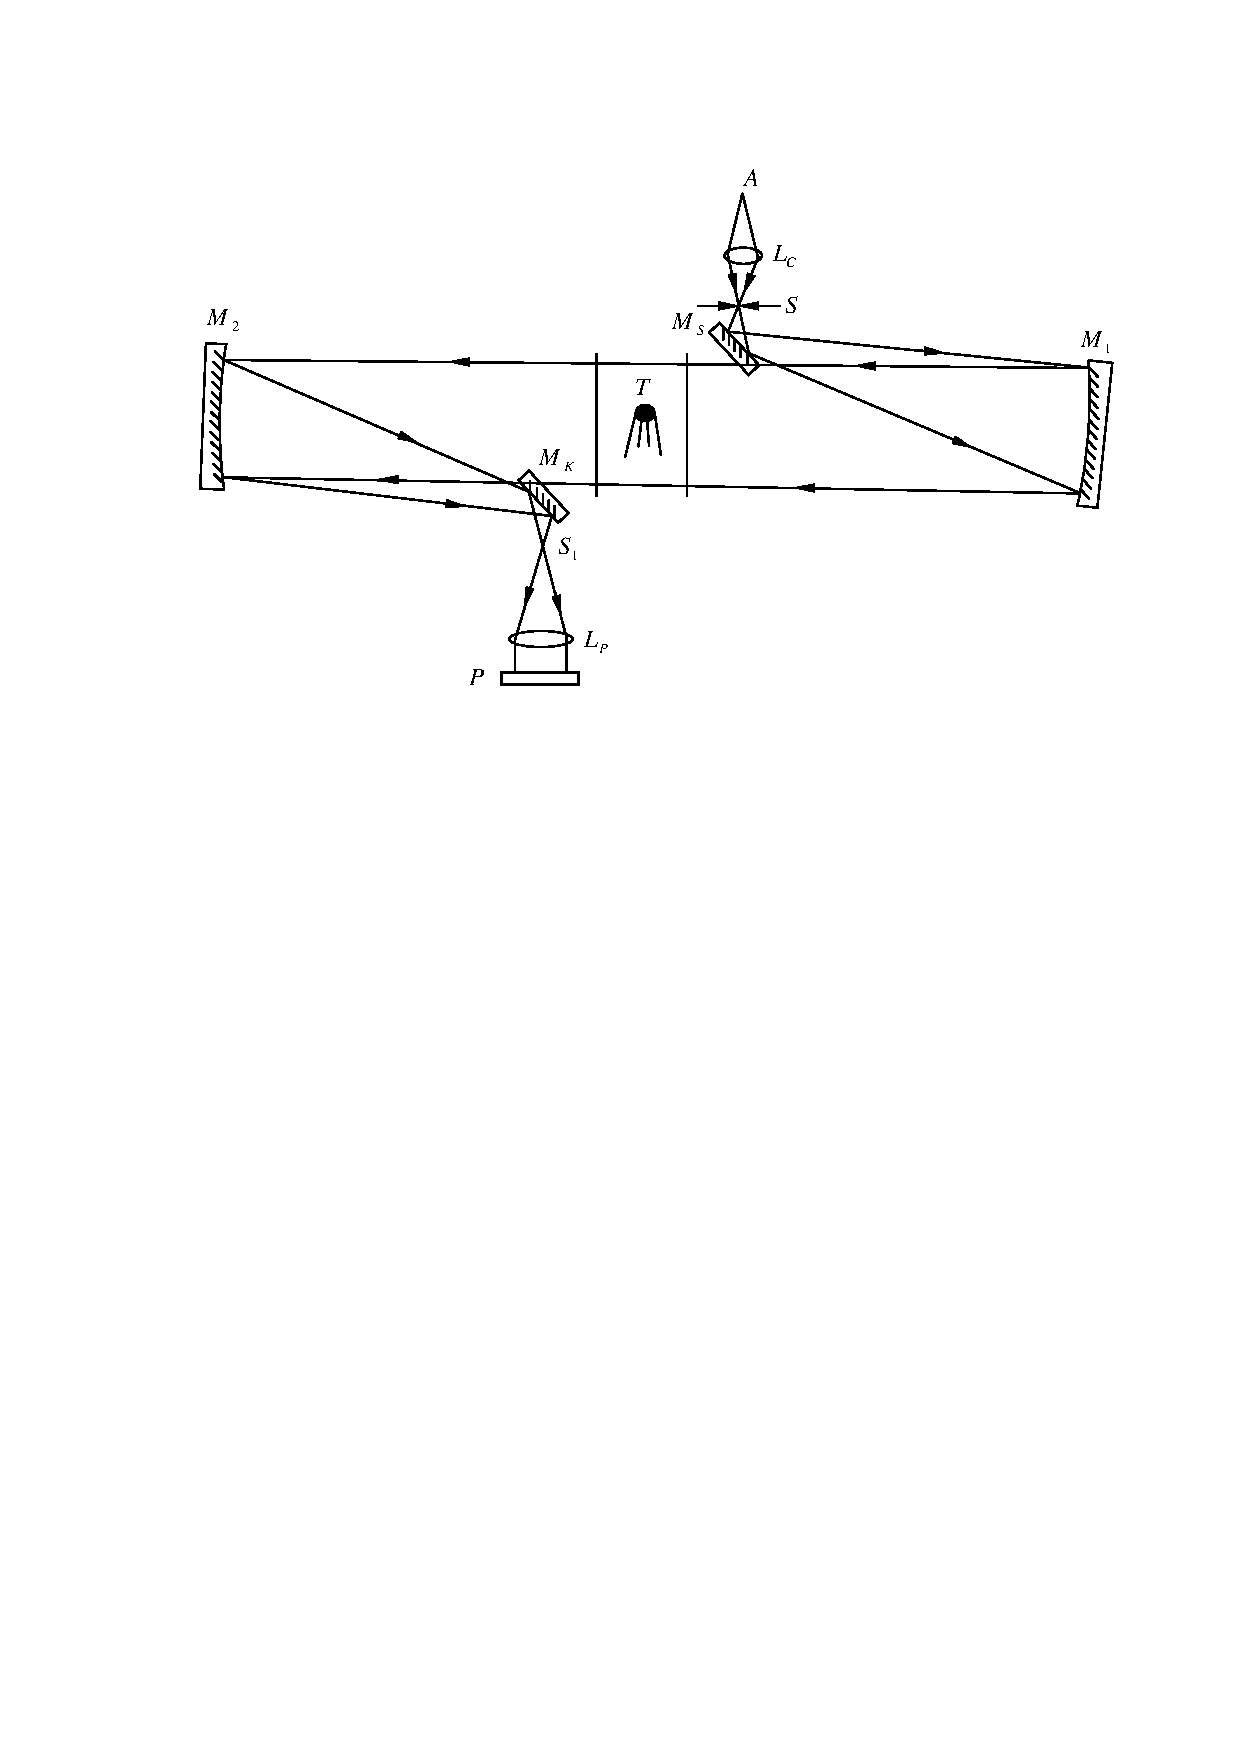
\includegraphics[width=0.7\textwidth]{shadow.pdf}
\caption{\label{shadow}平行光聚焦阴影系统}
\end{figure}
点光源$A$发出的光线由聚光系统$L_C$形成二次有效光源$S$, 在$S$平面上设置阴影小孔光阑, 根据灵敏度的不同要求, 确定小孔光阑直径的大小. 从$S$发出的光束, 由小反射镜$M_S$和球面镜 $M_1$反射, 形成平行光, 光束经过试验段$T$后, 由球面镜$M_2$会聚, 经过小反射镜$M_K$, 形成光源像$S_1$, 利用照相物镜$L_P$对流动区域成像, 得到清晰的阴影图$P$.

\subsection{纹影法}
纹影图一般可在阴影仪上获得, 只须在阴影仪焦平面上添加空间滤波元件刀口即可, 如图\ref{schlieren}所示.
\begin{figure}[!htb]
\centering
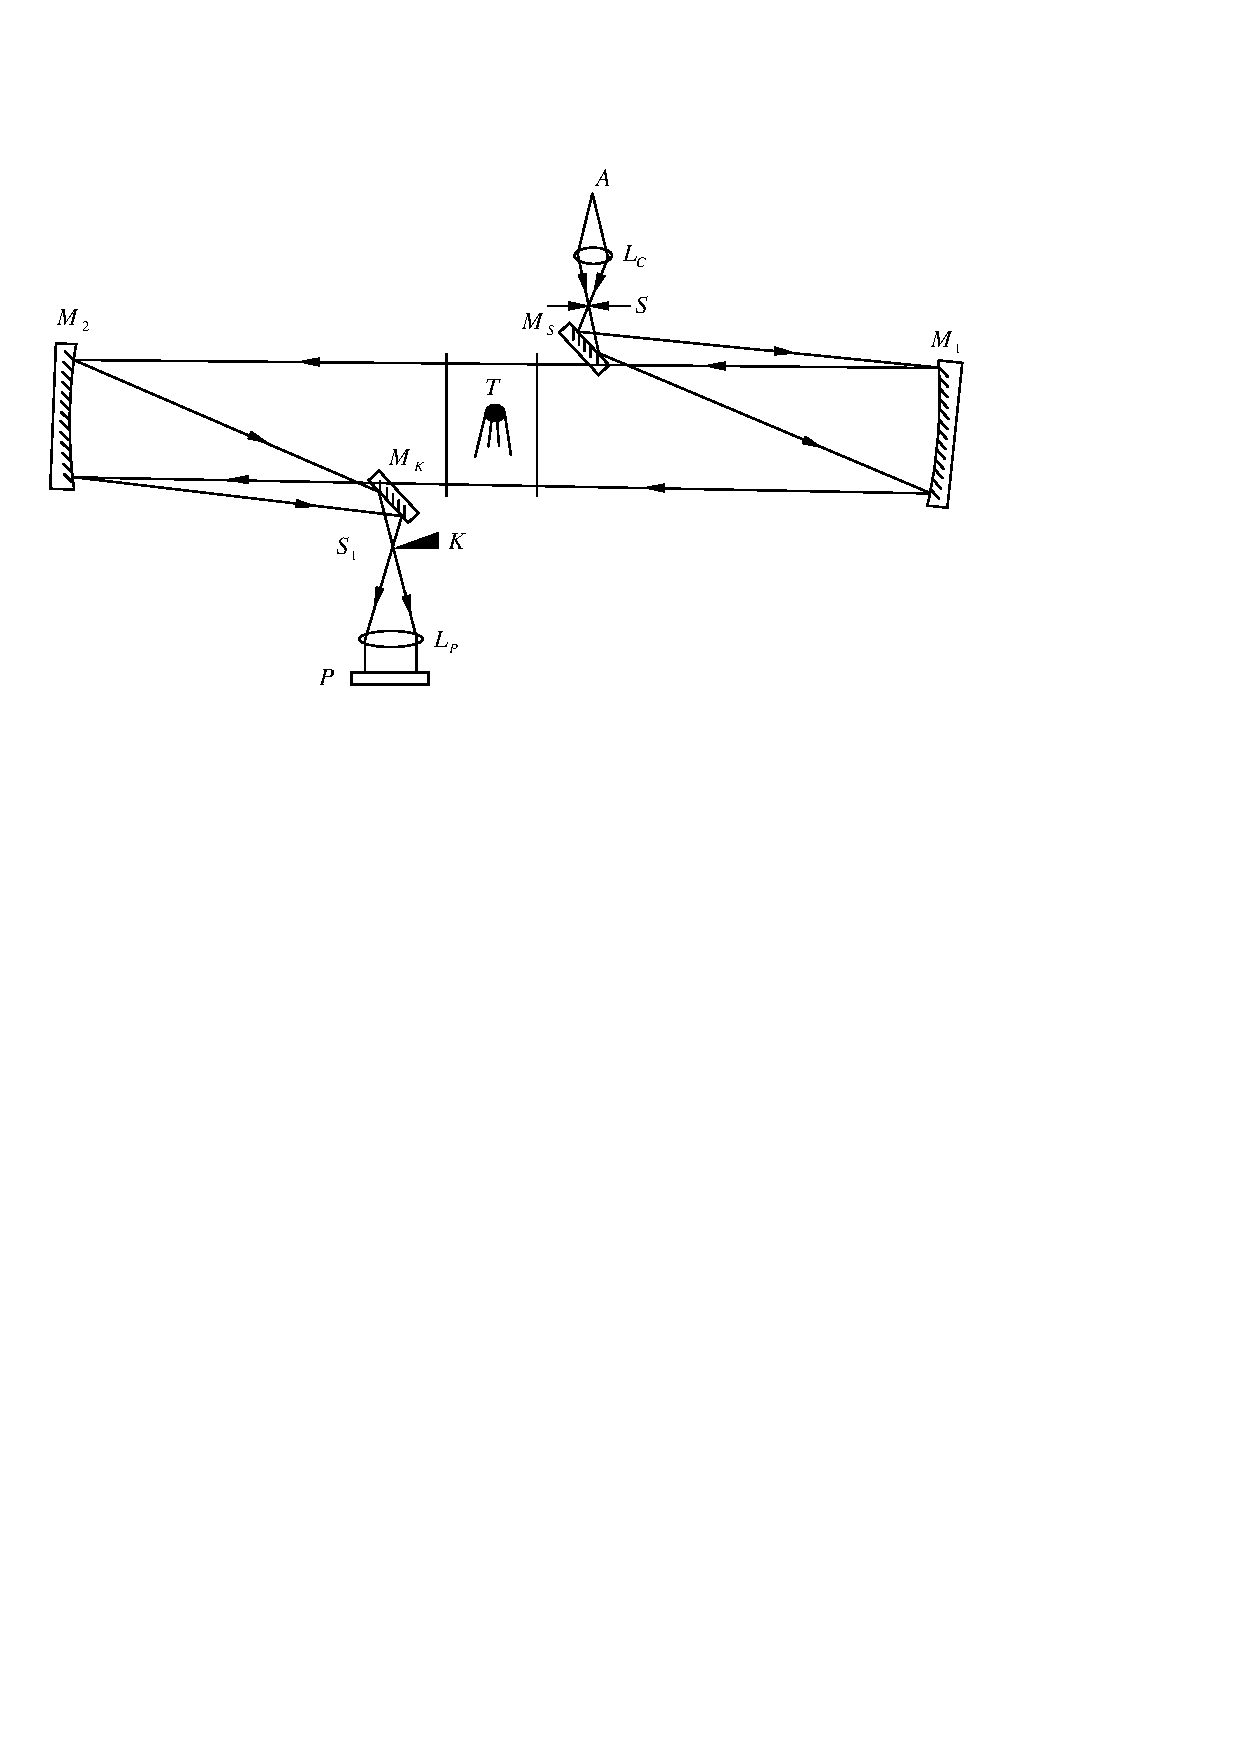
\includegraphics[width=0.7\textwidth]{schlieren.pdf}
\caption{\label{schlieren}双镜平行光纹影系统}
\end{figure}
点光源$A$发出的光线由聚光系统$L_C$会聚在小孔$S$的平面上, 经过小反射镜 $M_S$转折, 光束投射到纹影镜$M_1$上, 形成平行光, 光束经过试验段$T$后, 由纹影镜$M_2$聚焦, 经过小反射镜 $M_K$转折, 会聚在刀口$K$平面上, 在刀口平面上形成一个光源小孔像$S_1$, 被刀口切割后进入照相物镜$L_P$, 在底片平面$P$上成像.

\section{实验步骤及注意事项}
了解本实验的背景及阴影法和纹影法测流场的光学原理后, 具体进行实验操作时主要有以下几个具体步骤:
\begin{enumerate}
\item 按照实验光路图调节光路: 找到光源经凸透镜折射后的焦点, 在焦点处放置$S$平面上的小孔光阑, 形成点光源; 用小反射镜$M_S$将透过小孔的光反射到凹透镜$M_1$上,调节$M_1$的位置和俯仰角度, 形成平行光, 且使光尽量覆盖风洞实验段$T$; 调节小反射镜$M_K$的位置, 找到点光源的像$S_1$, 调节照相物镜$L_P$的位置和焦距, 直至$L_P$拍摄的照片清晰.
\item 安装CCD并与计算机正确连接, 接通电源, 打开LIVE3000应用软件, 即可在计算机显示器上观察到视场的图象.
\item 测试并调整CCD的触发与同步装置.
\item	把酒精灯放在光路中点燃, 调整CCD的焦距, 使图象清晰. 改变刀口的位置和方向, 观察图象有何差别. 可用计算机采集录影或单幅图象.
\item 先撤去刀口, 此时即为阴影法. 在实验段中通过一个马赫数为2.5的来流. 利用CCD照相观察流场的形态.	
\item 然后安装好刀口, 此时即为纹影法, 使用刀口分别纵切1/2, 3/4以及横切1/2. 同样在实验段中通过一个马赫数为2.5的来流, 利用CCD拍照观察流场的形态, 并与刚才阴影法的情况进行对比.
\end{enumerate}
\begin{figure}[!htb]
\begin{minipage}[b]{.5\textwidth}
\centering
\fbox{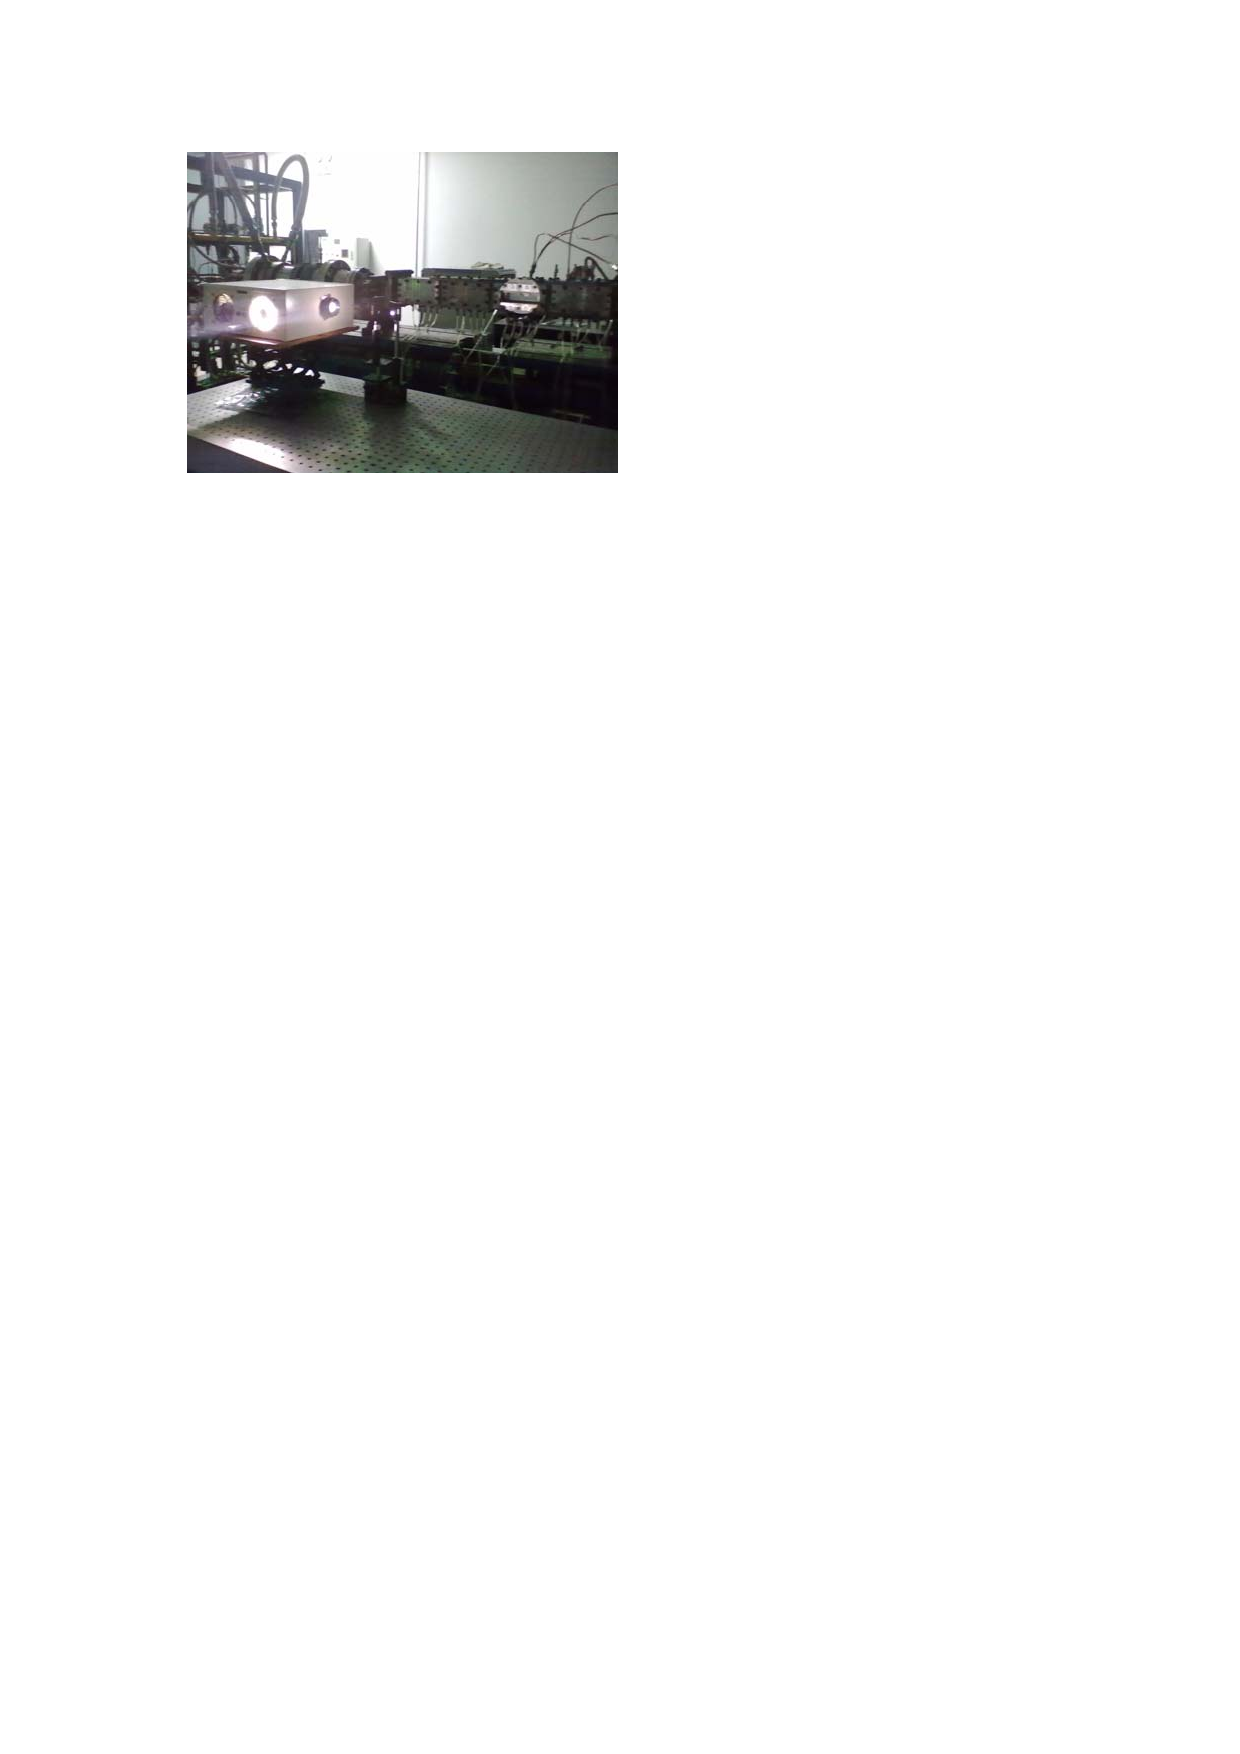
\includegraphics[width=0.8\textwidth]{ex01.pdf}}
\end{minipage}%
\begin{minipage}[b]{.5\textwidth}
\centering
\fbox{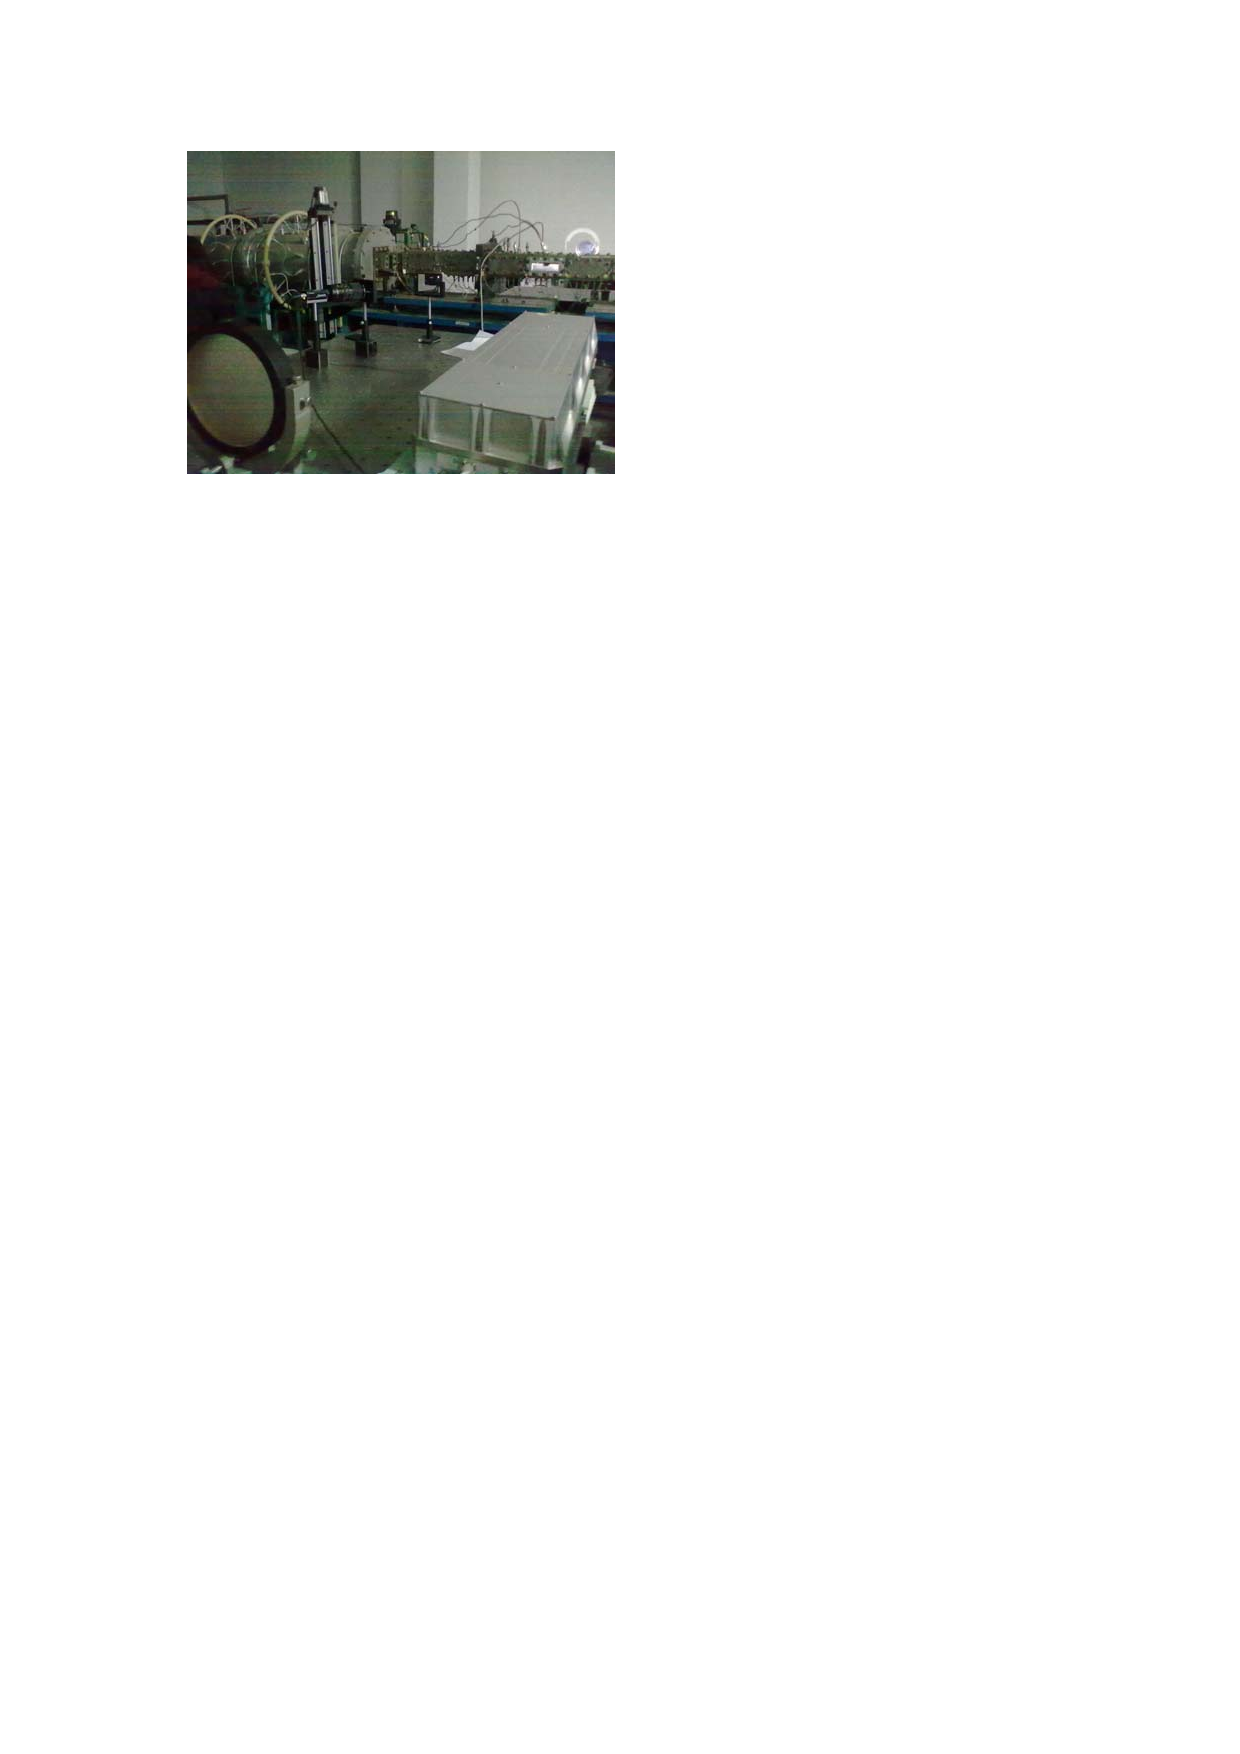
\includegraphics[width=0.8\textwidth]{ex02.pdf}}
\end{minipage}
\caption{\label{ex}实验中调试出的实验光路}
\end{figure}
以上实验步骤中, 还需要注意以下几点:
\begin{enumerate}
\item 对于阴影法, 由于平行光聚焦阴影系统是一个离轴光学系统, 离轴角$\theta_1$和$\theta_2$ 尽可能调整到相等, 从而减少离轴系统的相差.
\item 对于纹影法, 尽可能使光源小孔像$S_1$与刀口$K$在同一平面内,减少反射镜$M_1$和$M_2$的离轴工作带来的彗差和像散.
\item 由于球面反射镜表面镀膜, 实验过程中不可用手触摸或擦拭镜面, 以免损坏表面镀层.
\end{enumerate}

\section{实验结果及分析}
\subsection{实验结果}

图\ref{fire}和图\ref{wave}显示的分别为阴影法及纹阴法下纵向切去1/2, 3/4光线及横向切去1/4光线的火焰图案和激波图案. 从图\ref{fire}中可以看出纹影法获得到流场图案较阴影法的暗, 且``刀口''切去的光线越多, 图案越暗.
纹影图有明暗相间的条纹, 显示的细节比较多, 而阴影图除了显示火焰的边界, 流场其他地方基本一样.
并且通过观察图, 可以看到火焰边缘为亮纹, 根据阴影法原理屏幕上亮度的变化正比于密度的二阶导数, 当$\partial^2/\partial x^2>0$
时, 光线的偏转有发散的趋势(形成暗区); 反之有聚拢的趋势(形成亮区).
此时$\partial^2\rho/\partial x^2 <0$, $\partial\rho/\partial x$由大变小, 外焰温度高于周边空气和内焰.
\begin{figure}[!htb]
\begin{minipage}[b]{.5\textwidth}
\centering
\fbox{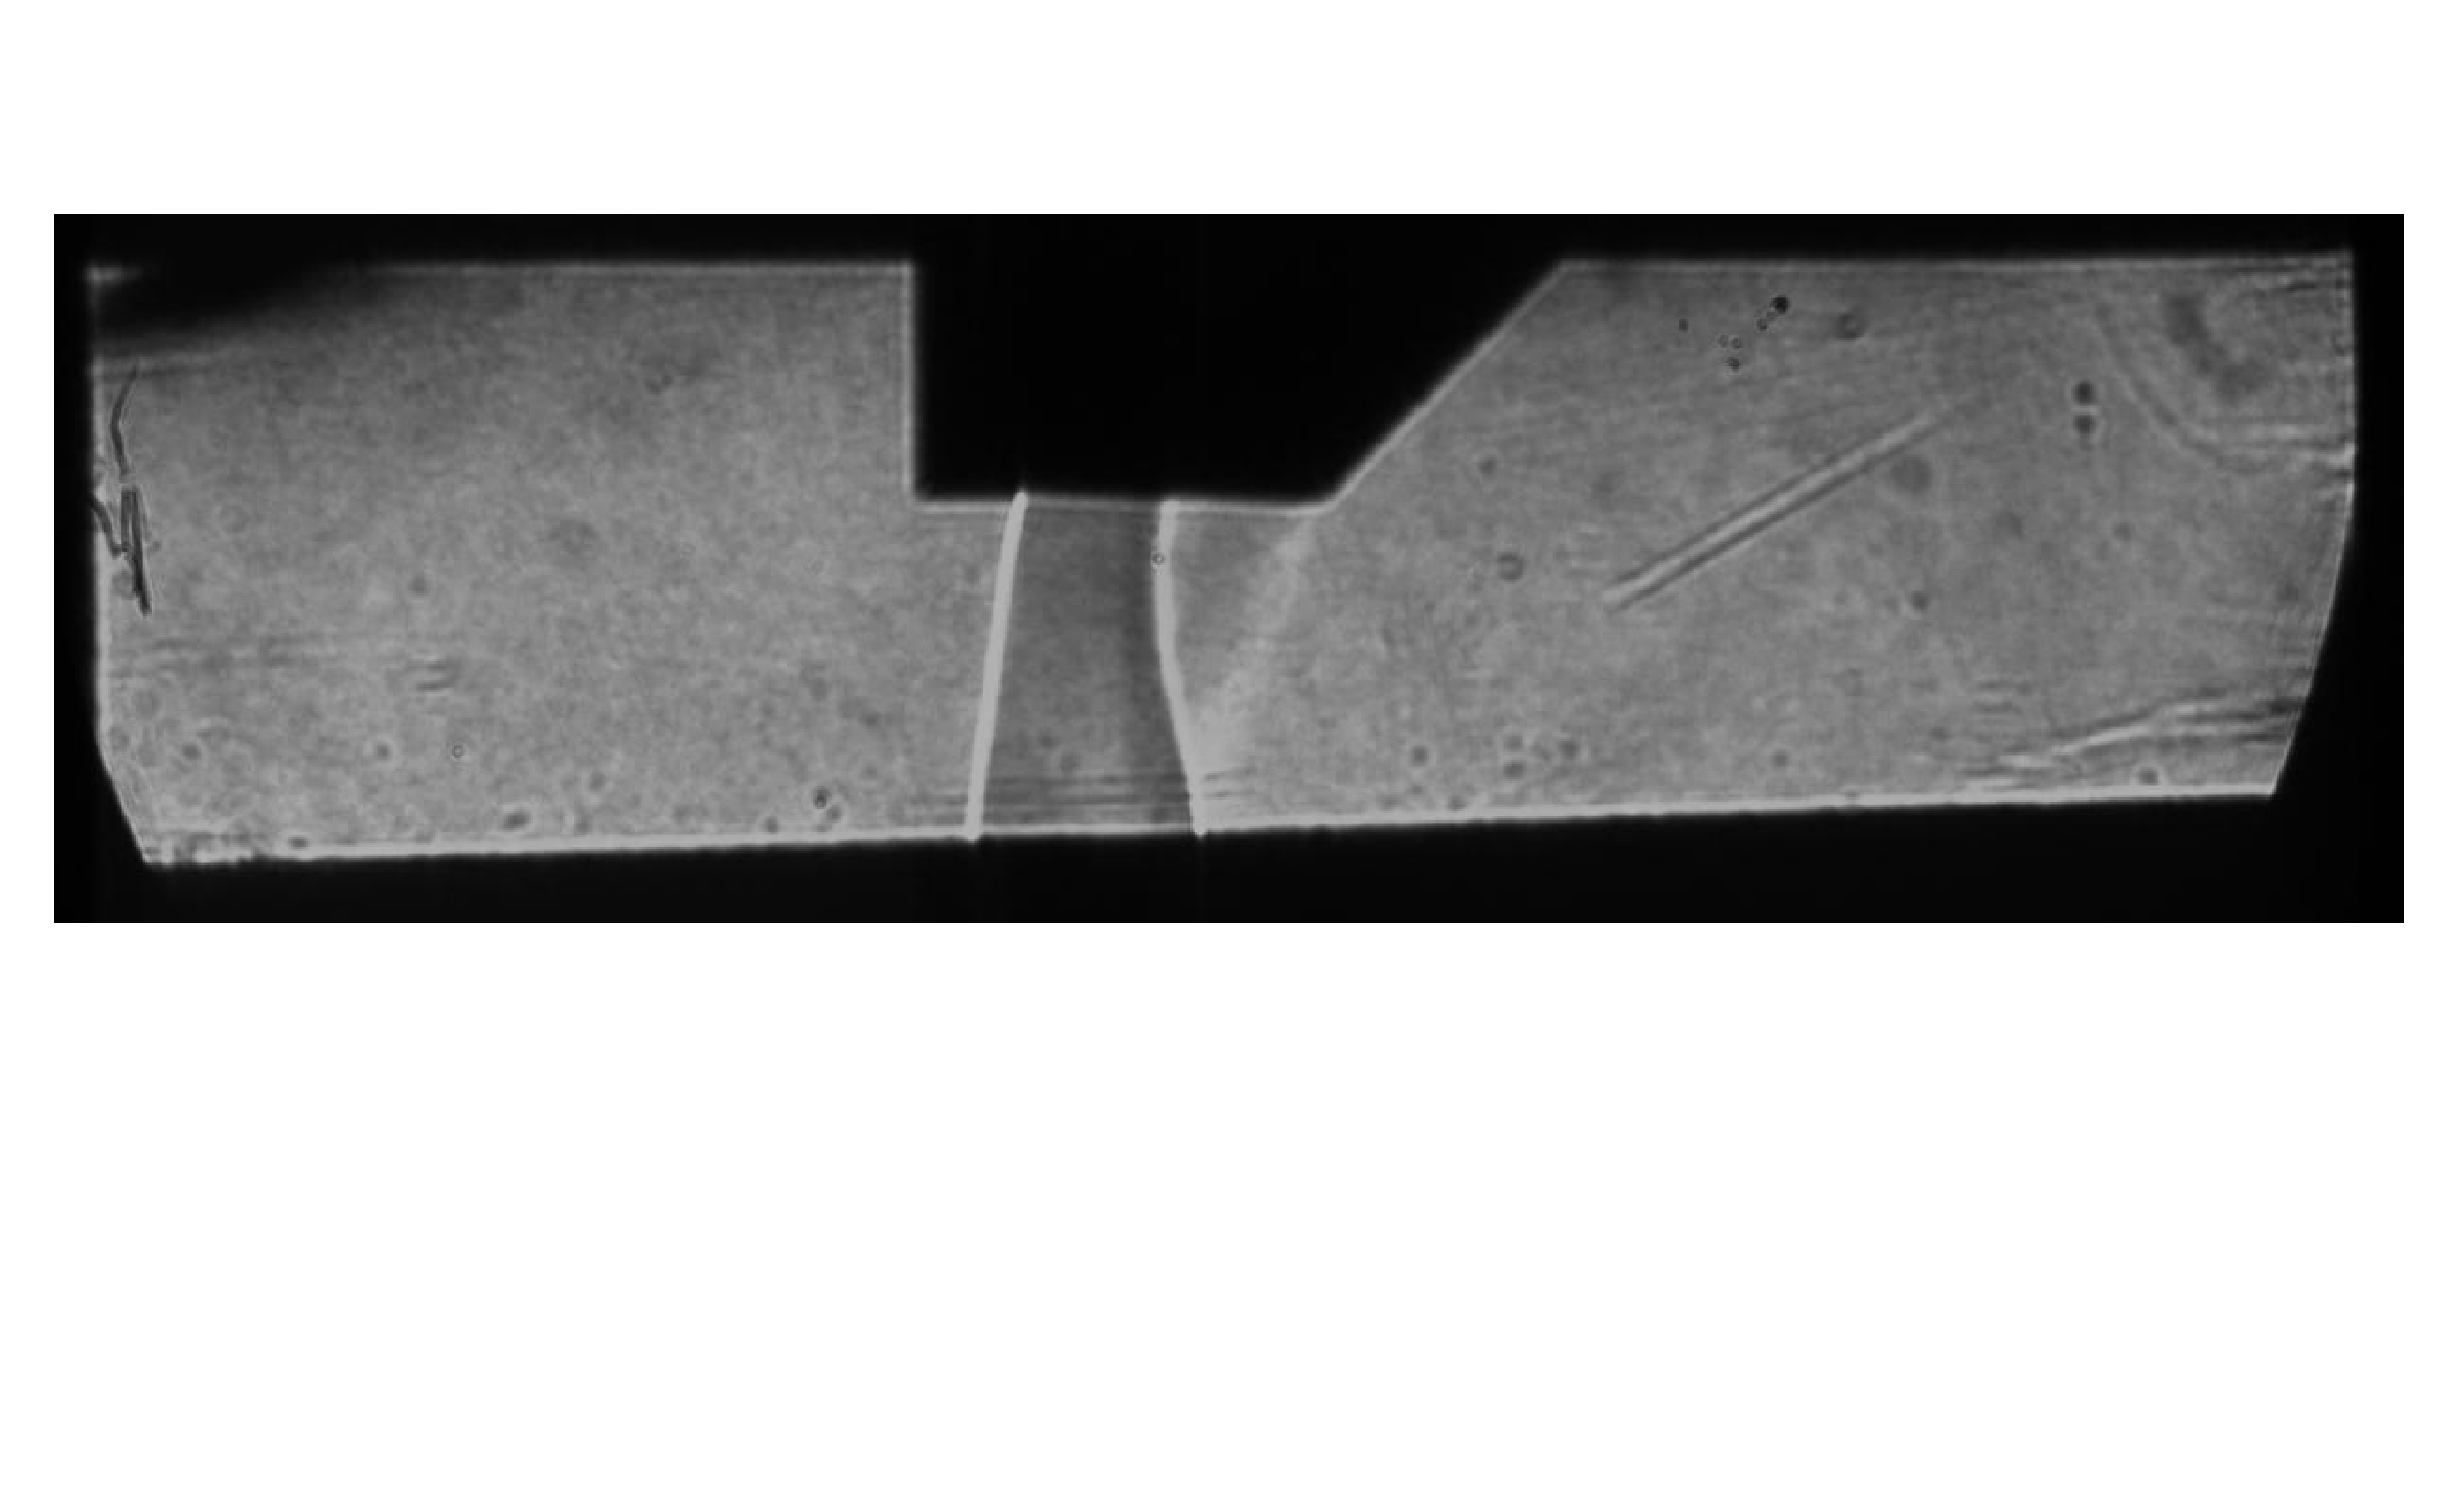
\includegraphics[width=0.95\textwidth]{shadow1of2.pdf}}\\
(a)阴影法{\textcolor{white}{纵切1/2光线}}
\end{minipage}%
\begin{minipage}[b]{.5\textwidth}
\centering
\fbox{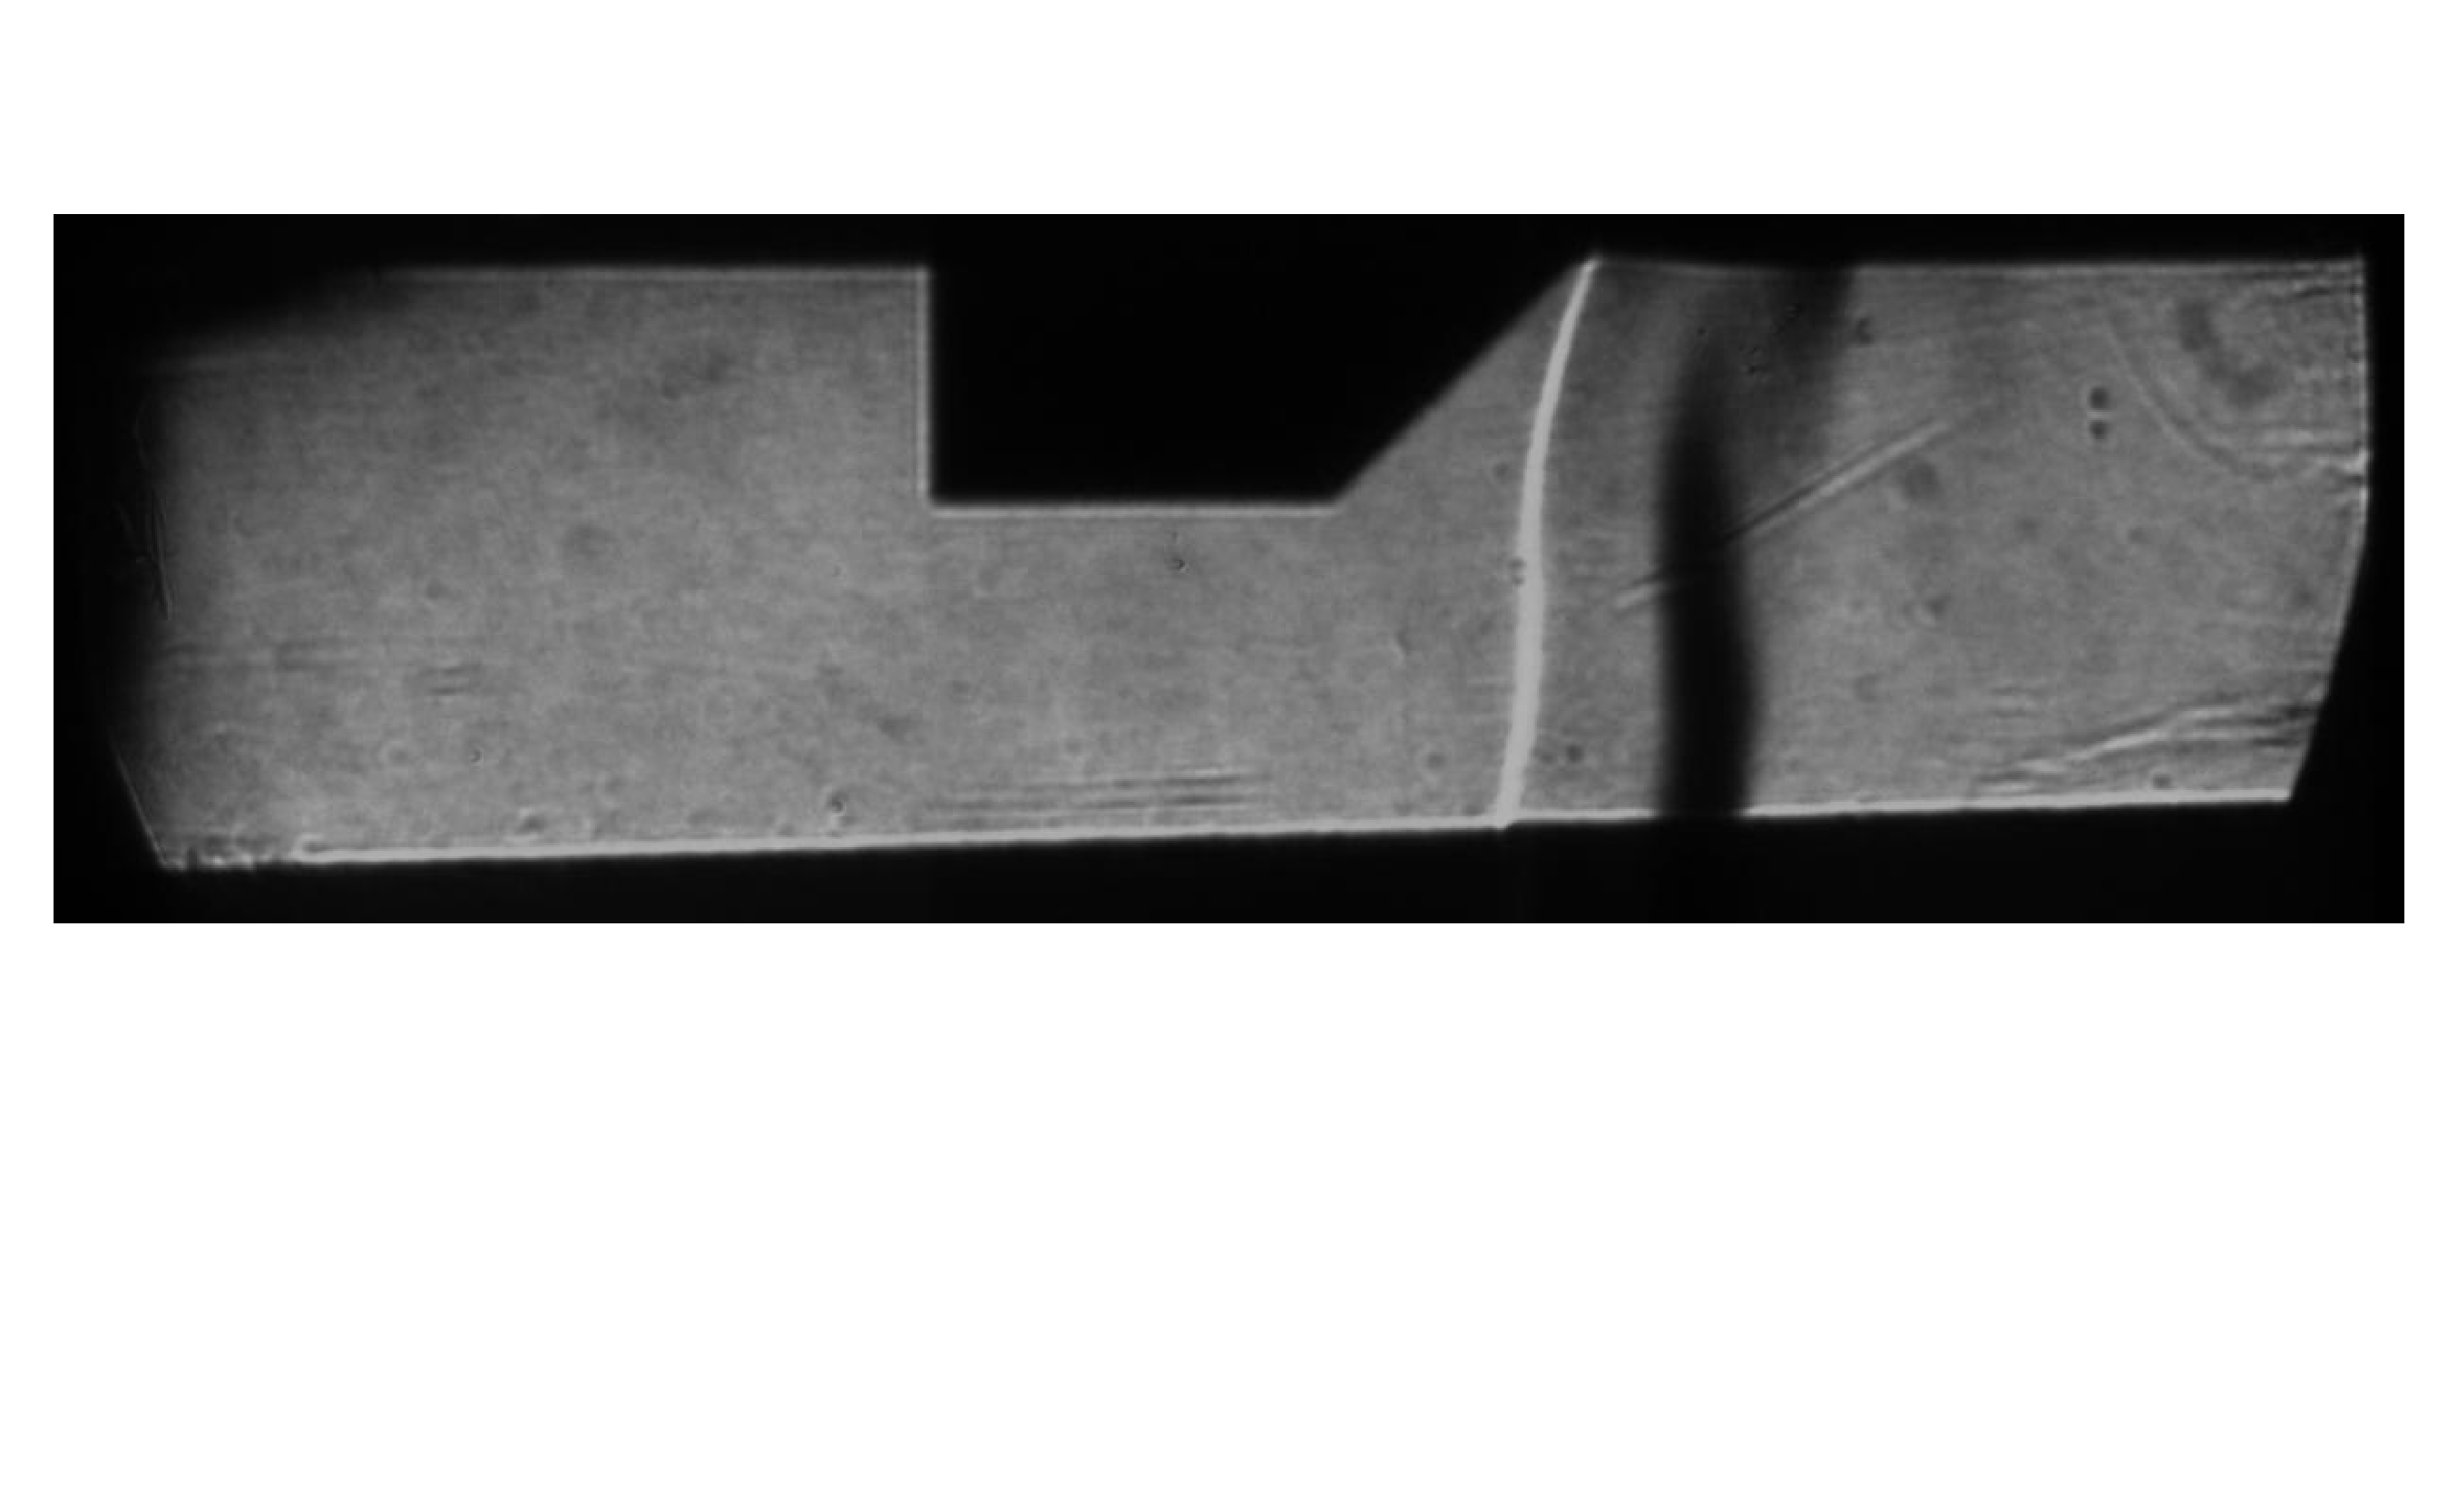
\includegraphics[width=0.95\textwidth]{fire-schlieren1of2.pdf}}\\
(b)纹影法纵切1/2光线
\end{minipage}
\\
\begin{minipage}[b]{.5\textwidth}
\centering
\fbox{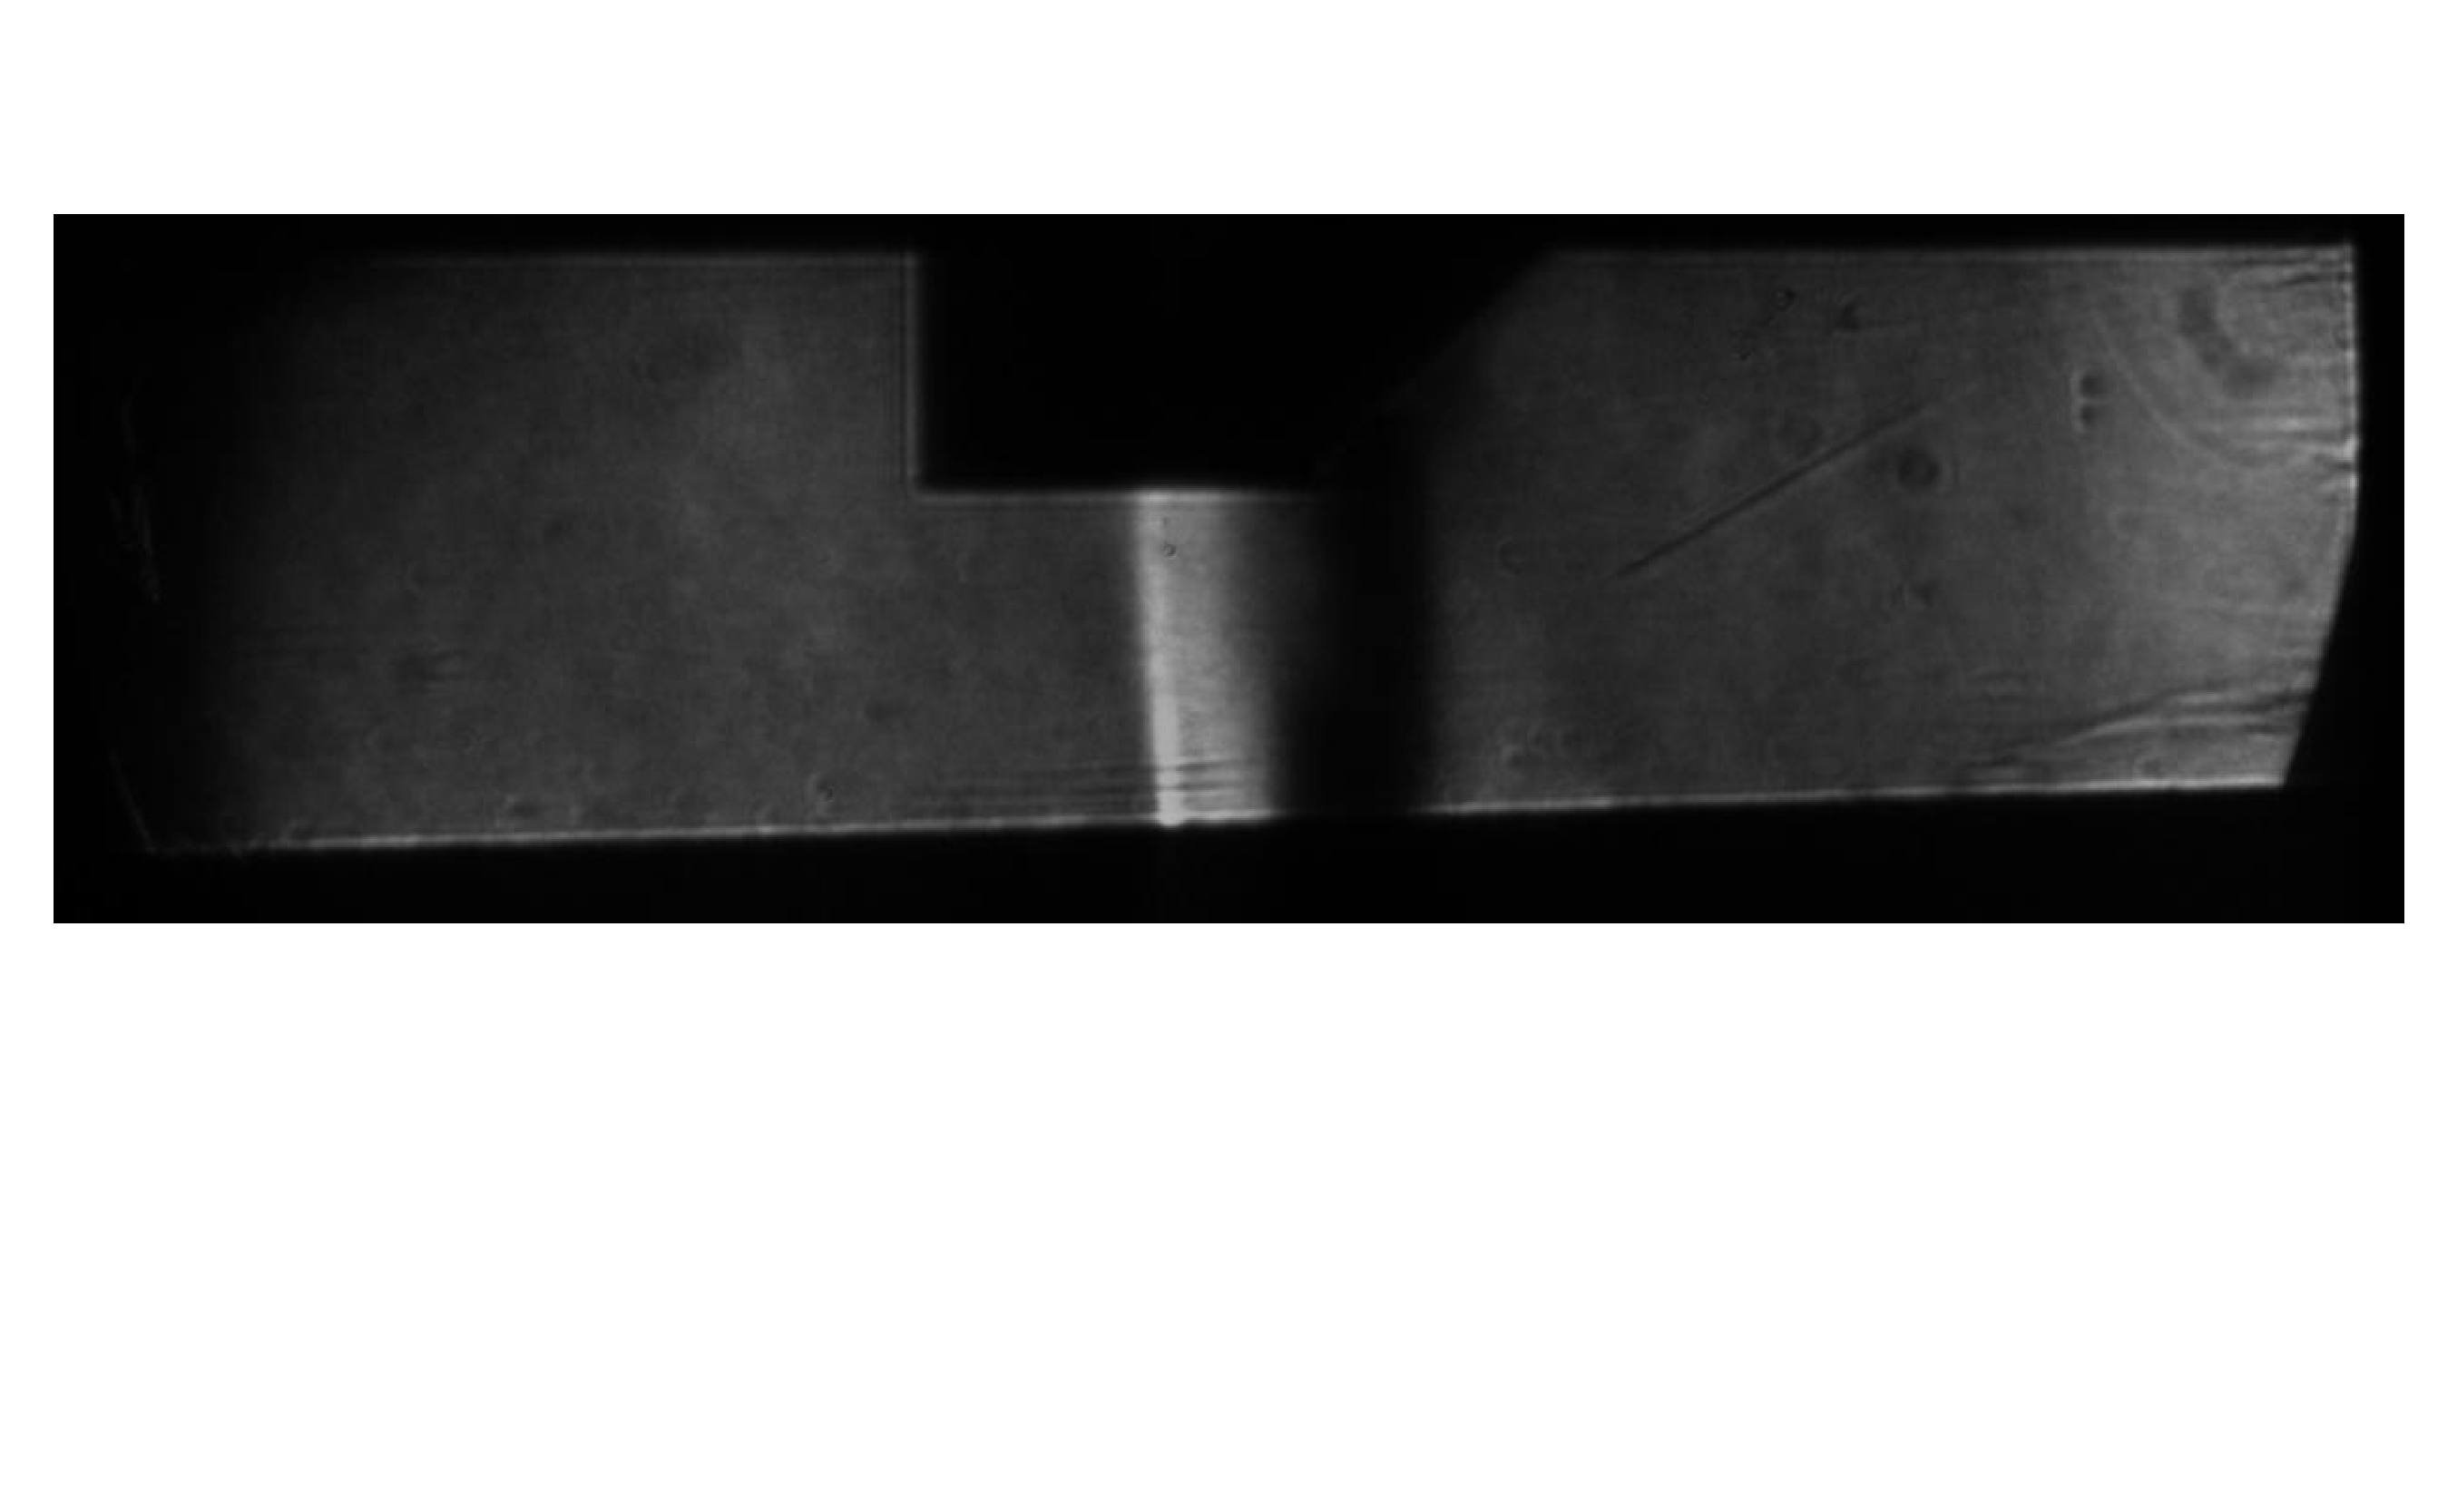
\includegraphics[width=0.95\textwidth]{fire-schlieren3of4.pdf}}\\
(c)纹影法纵切3/4光线
\end{minipage}%
\begin{minipage}[b]{.5\textwidth}
\centering
\fbox{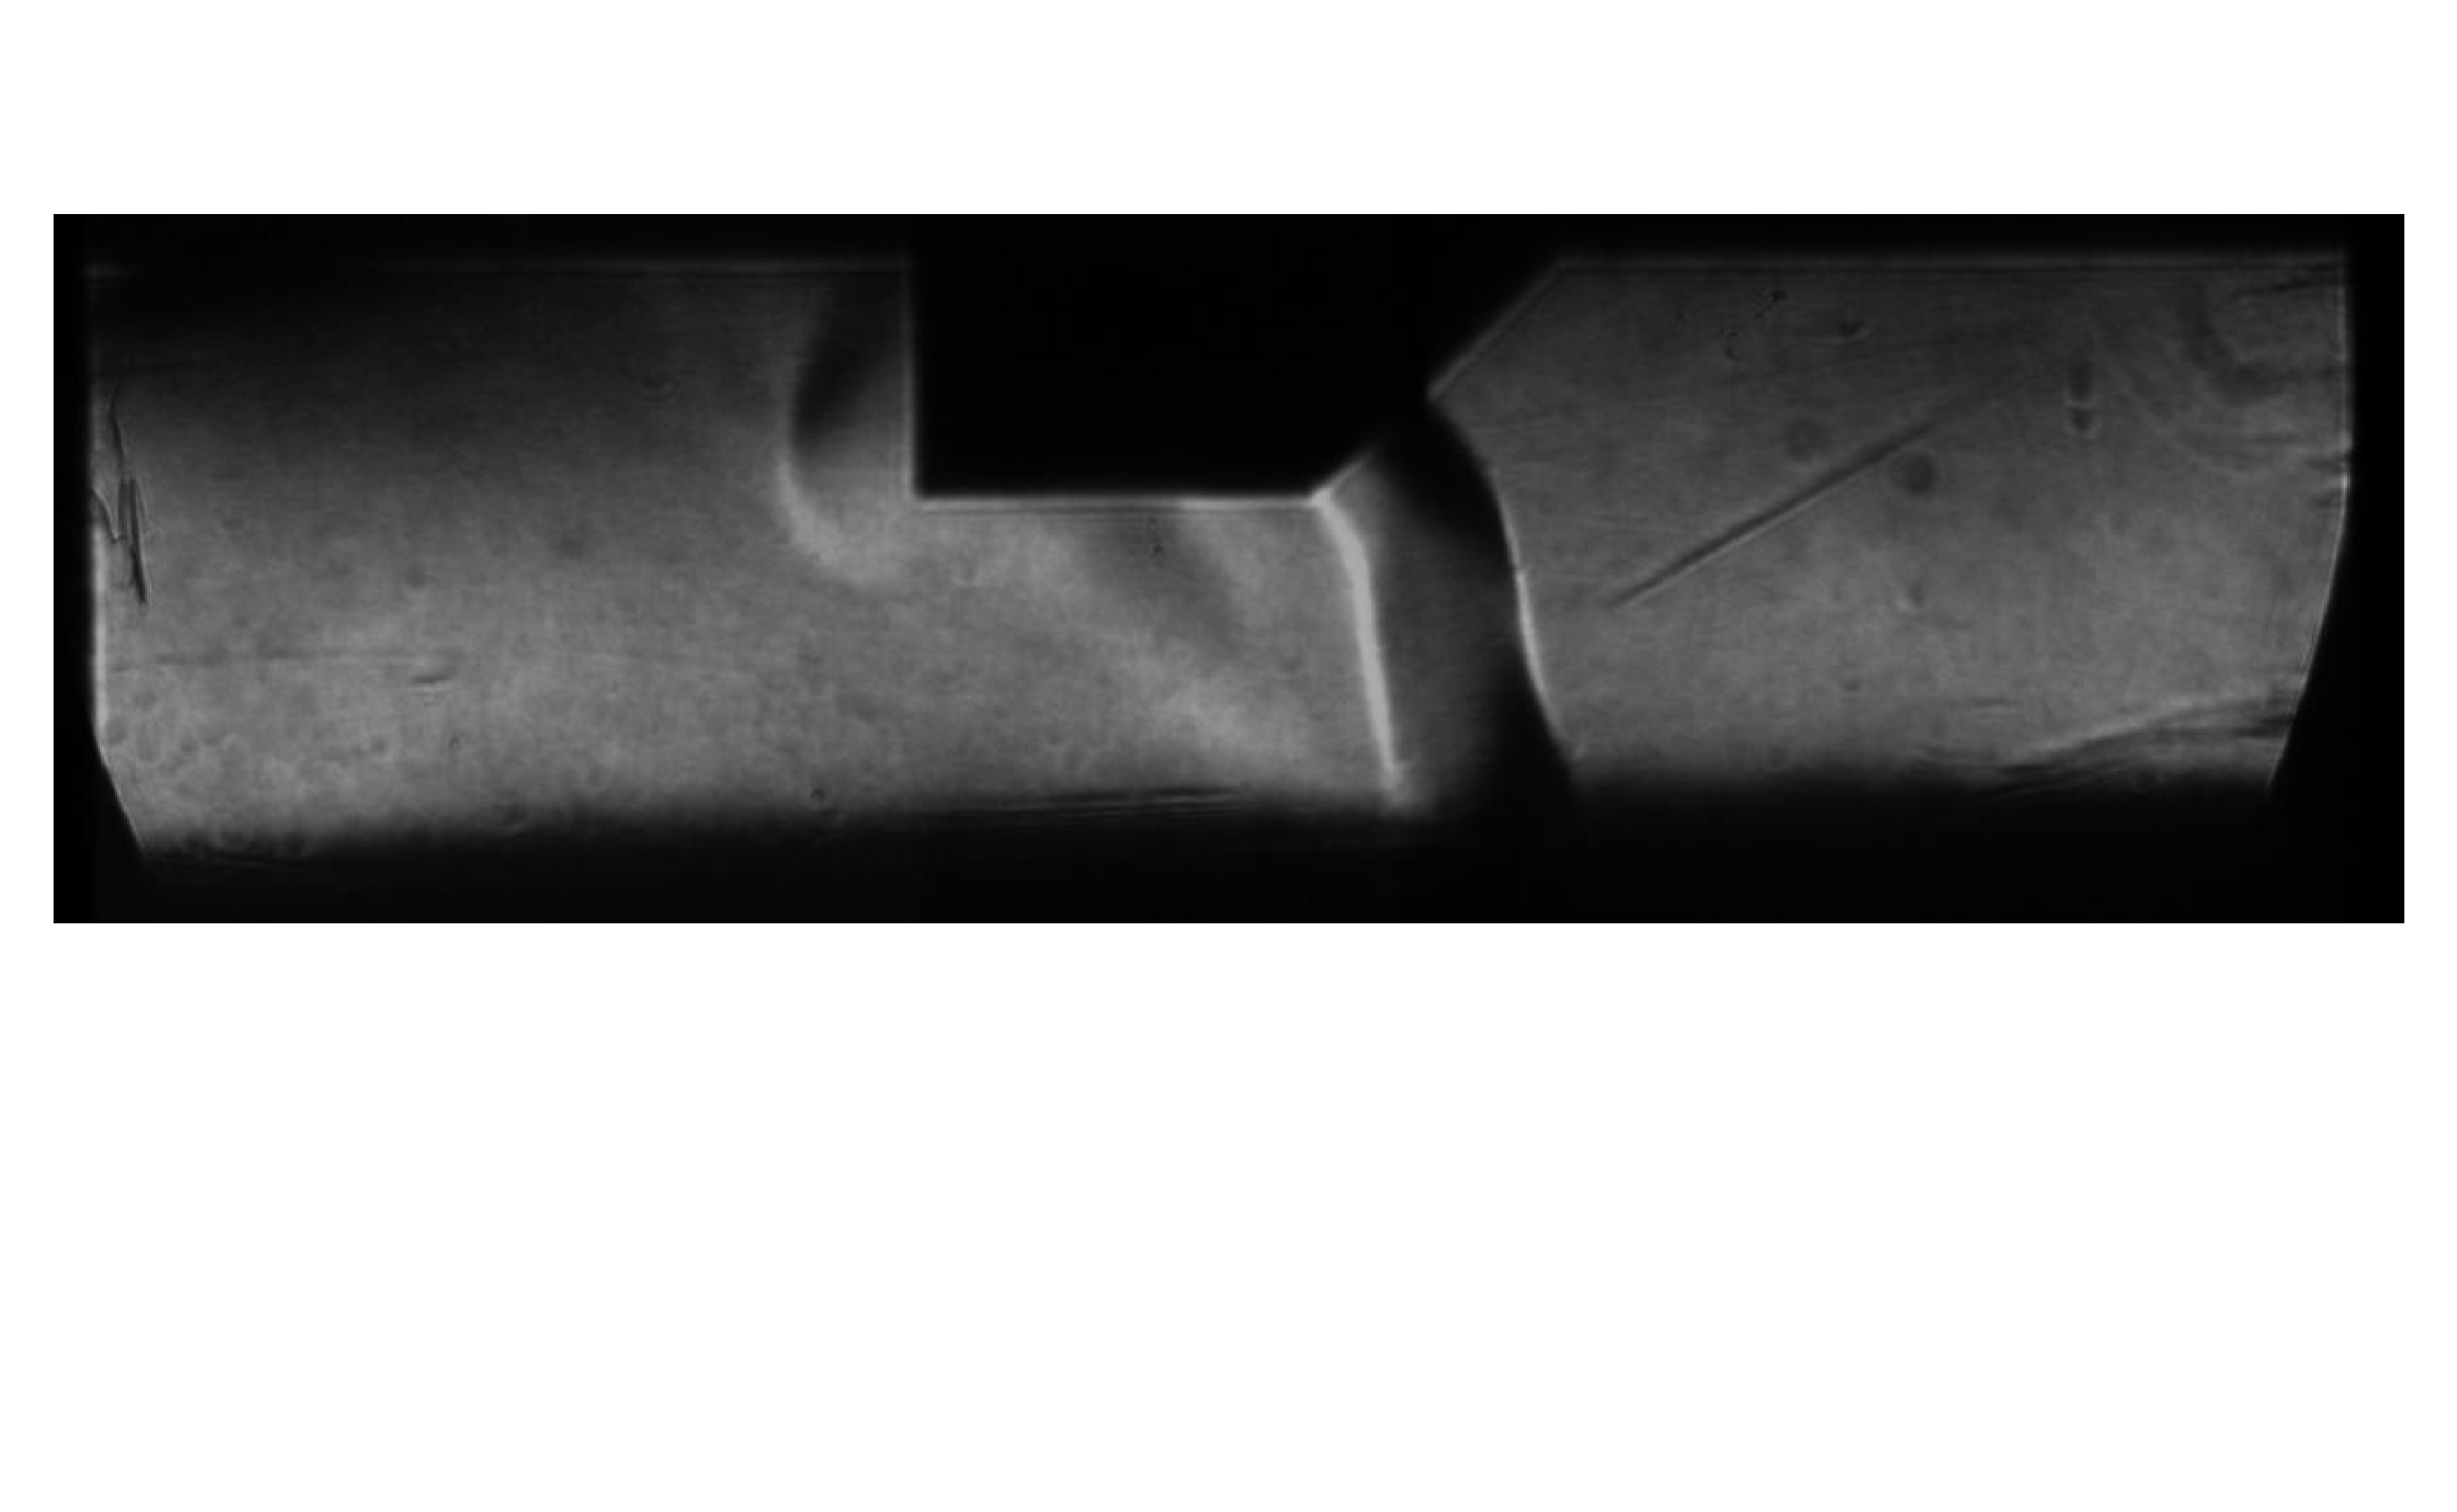
\includegraphics[width=0.95\textwidth]{fire-hschlieren1of2.pdf}}\\
(d)纹影法横切1/2光线
\end{minipage}
\caption{\label{fire}四种情况下的火焰图案}
\end{figure}
\begin{figure}[!htb]
\begin{minipage}[b]{.5\textwidth}
\centering
\fbox{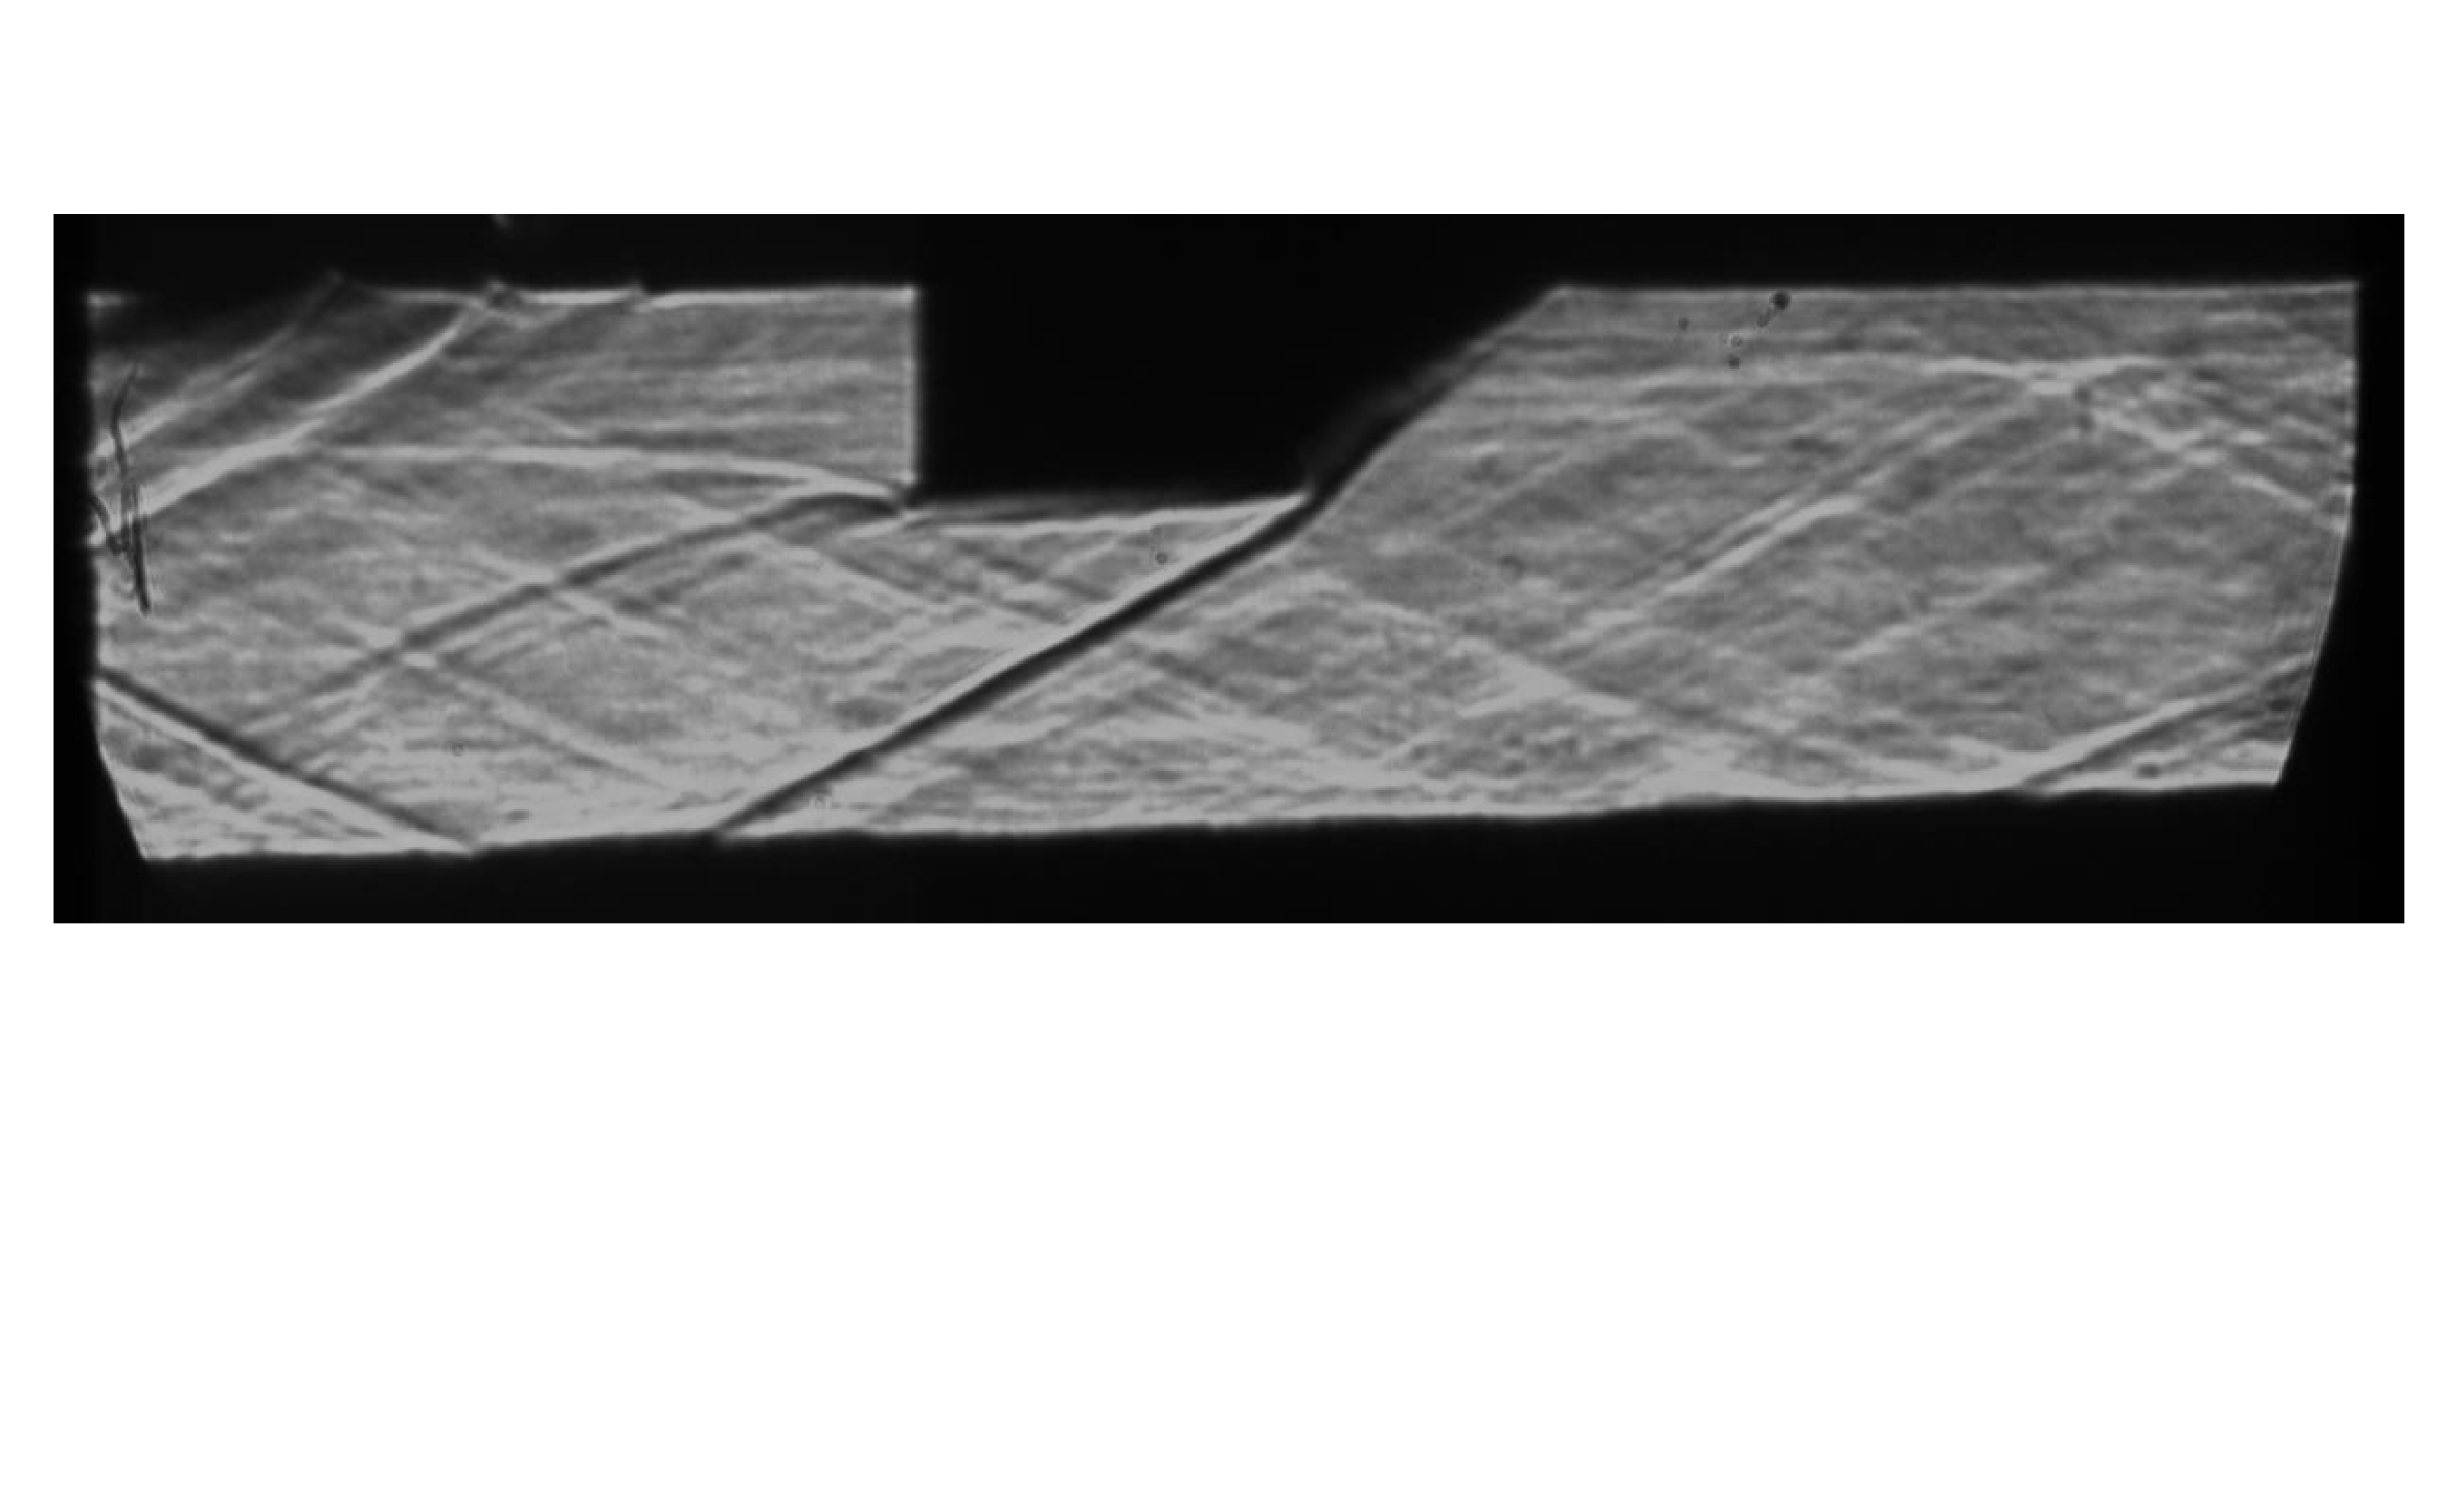
\includegraphics[width=0.95\textwidth]{WaveShadow.pdf}}\\
(a)阴影法{\textcolor{white}{纵切1/2光线}}
\end{minipage}%
\begin{minipage}[b]{.5\textwidth}
\centering
\fbox{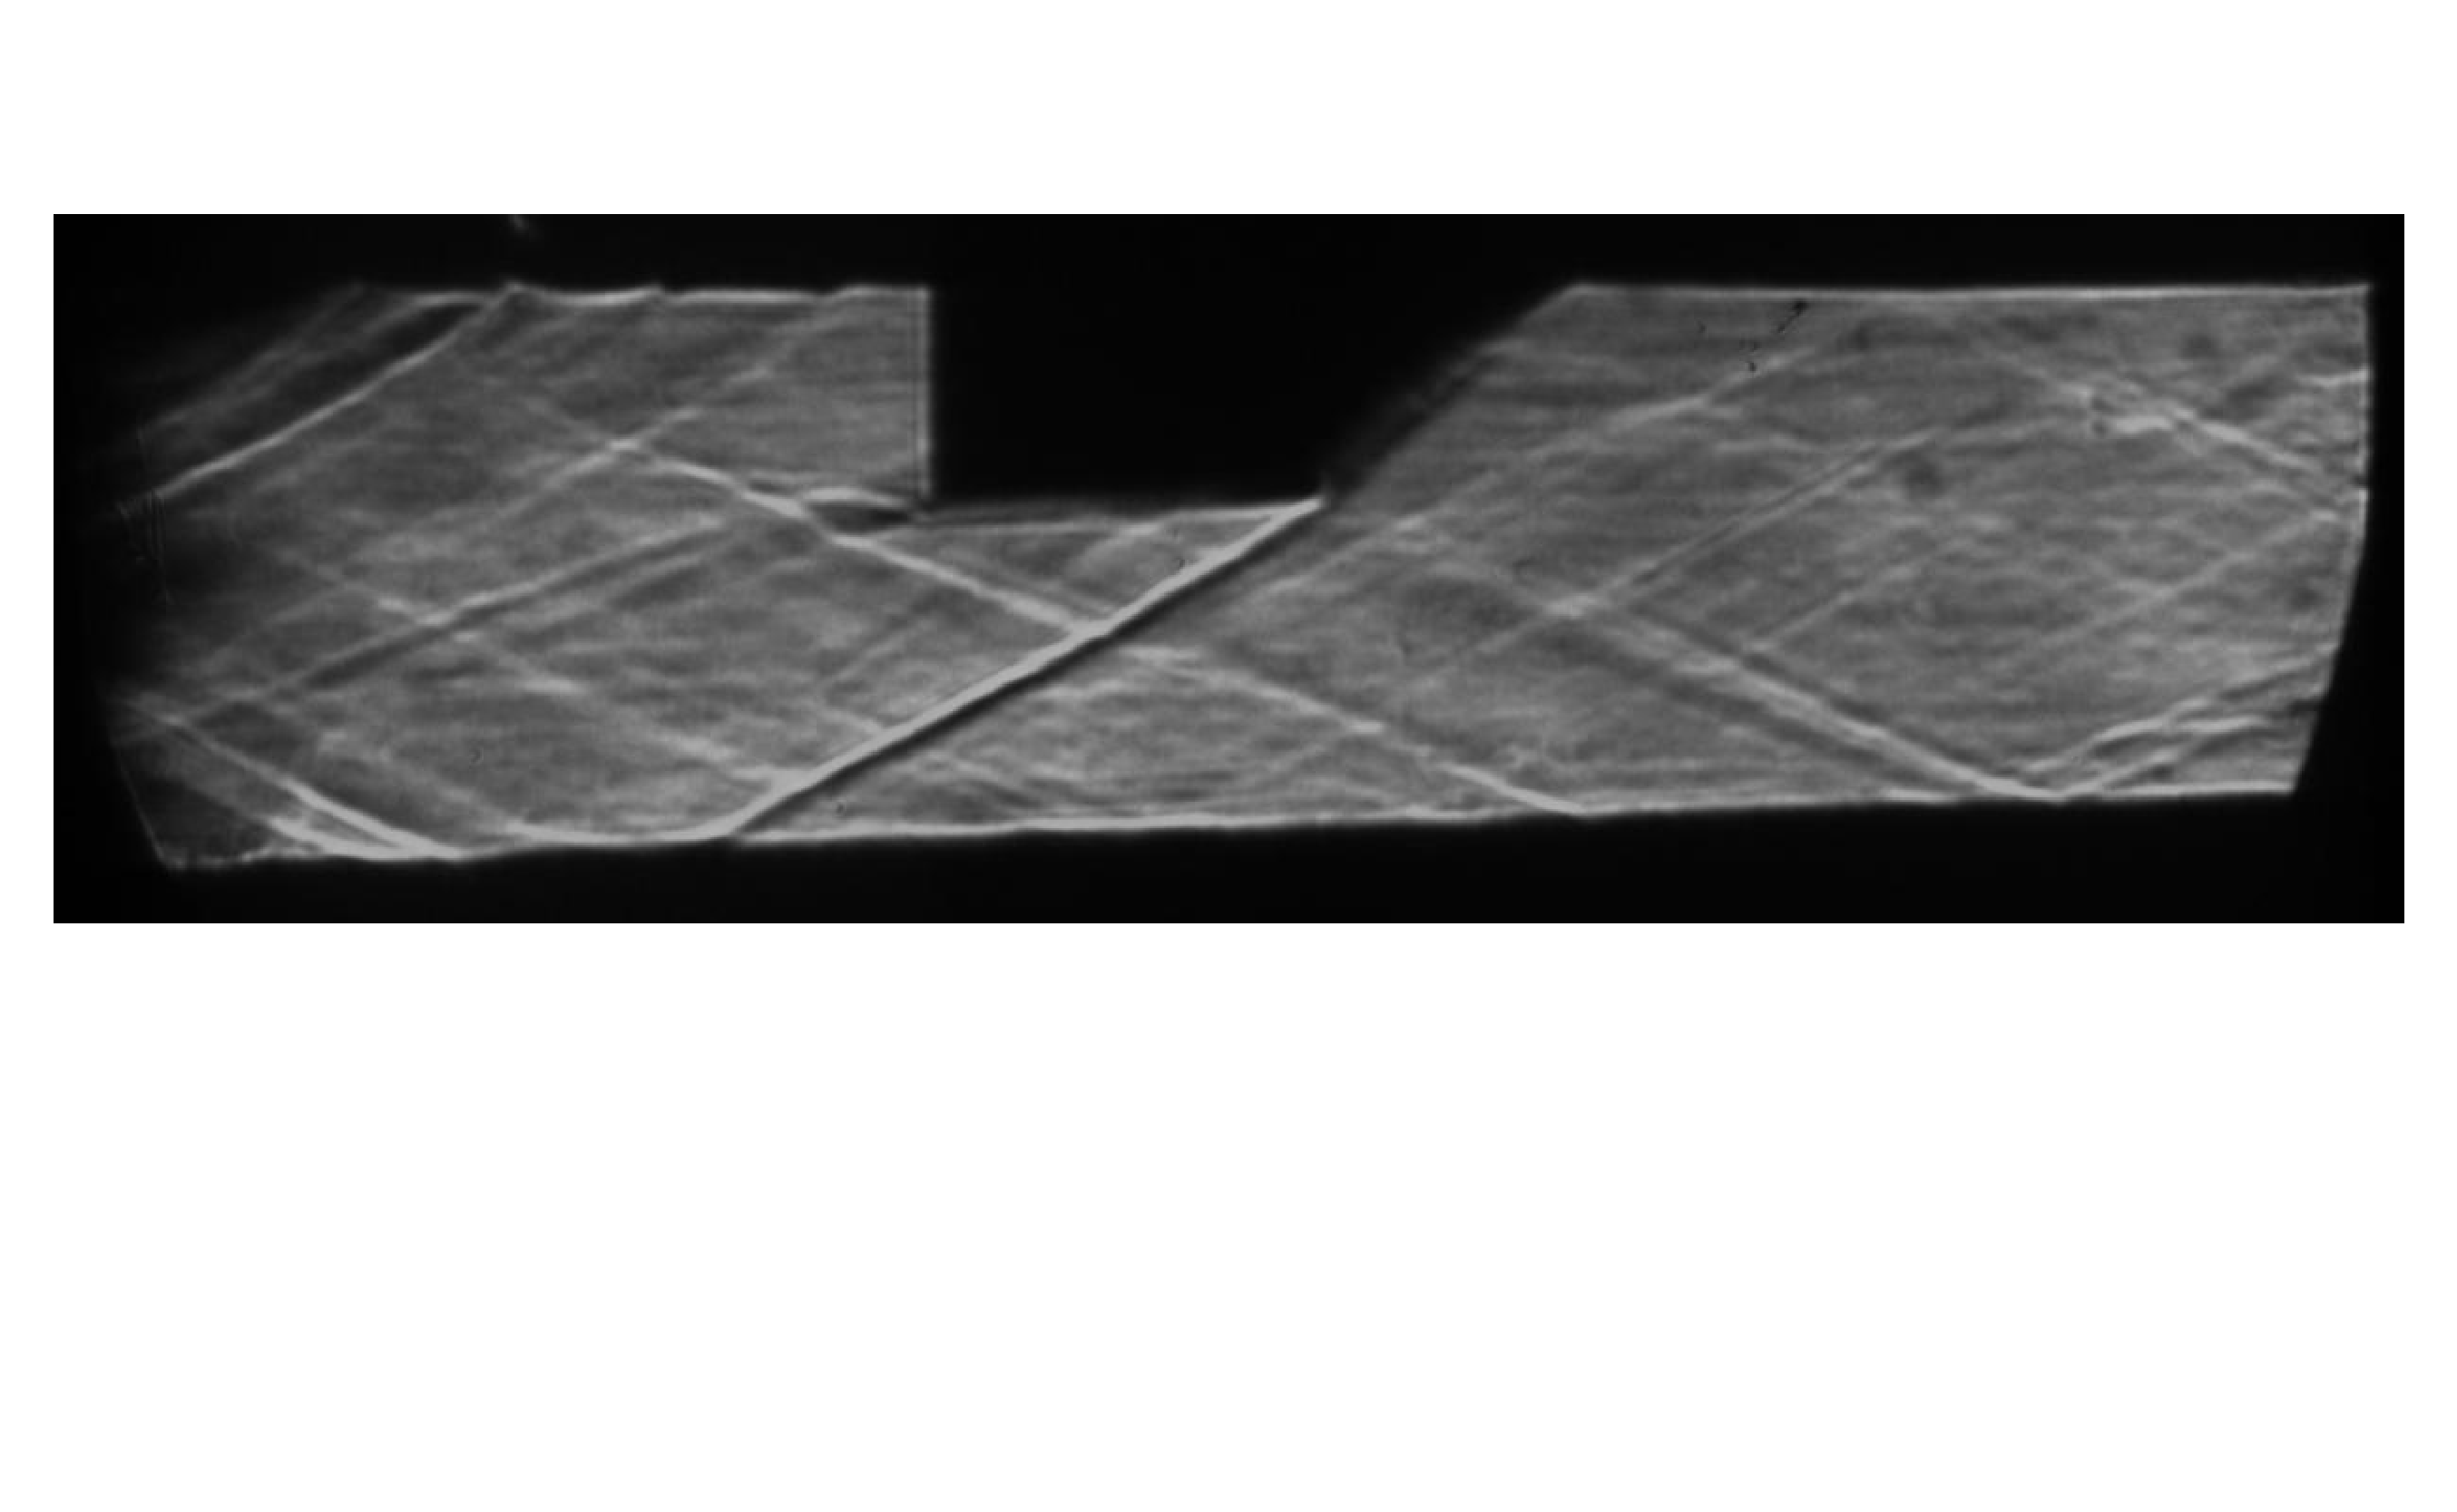
\includegraphics[width=0.95\textwidth]{WaveSchlieren1of2.pdf}}\\
(b)纹影法纵切1/2光线
\end{minipage}
\\
\begin{minipage}[b]{.5\textwidth}
\centering
\fbox{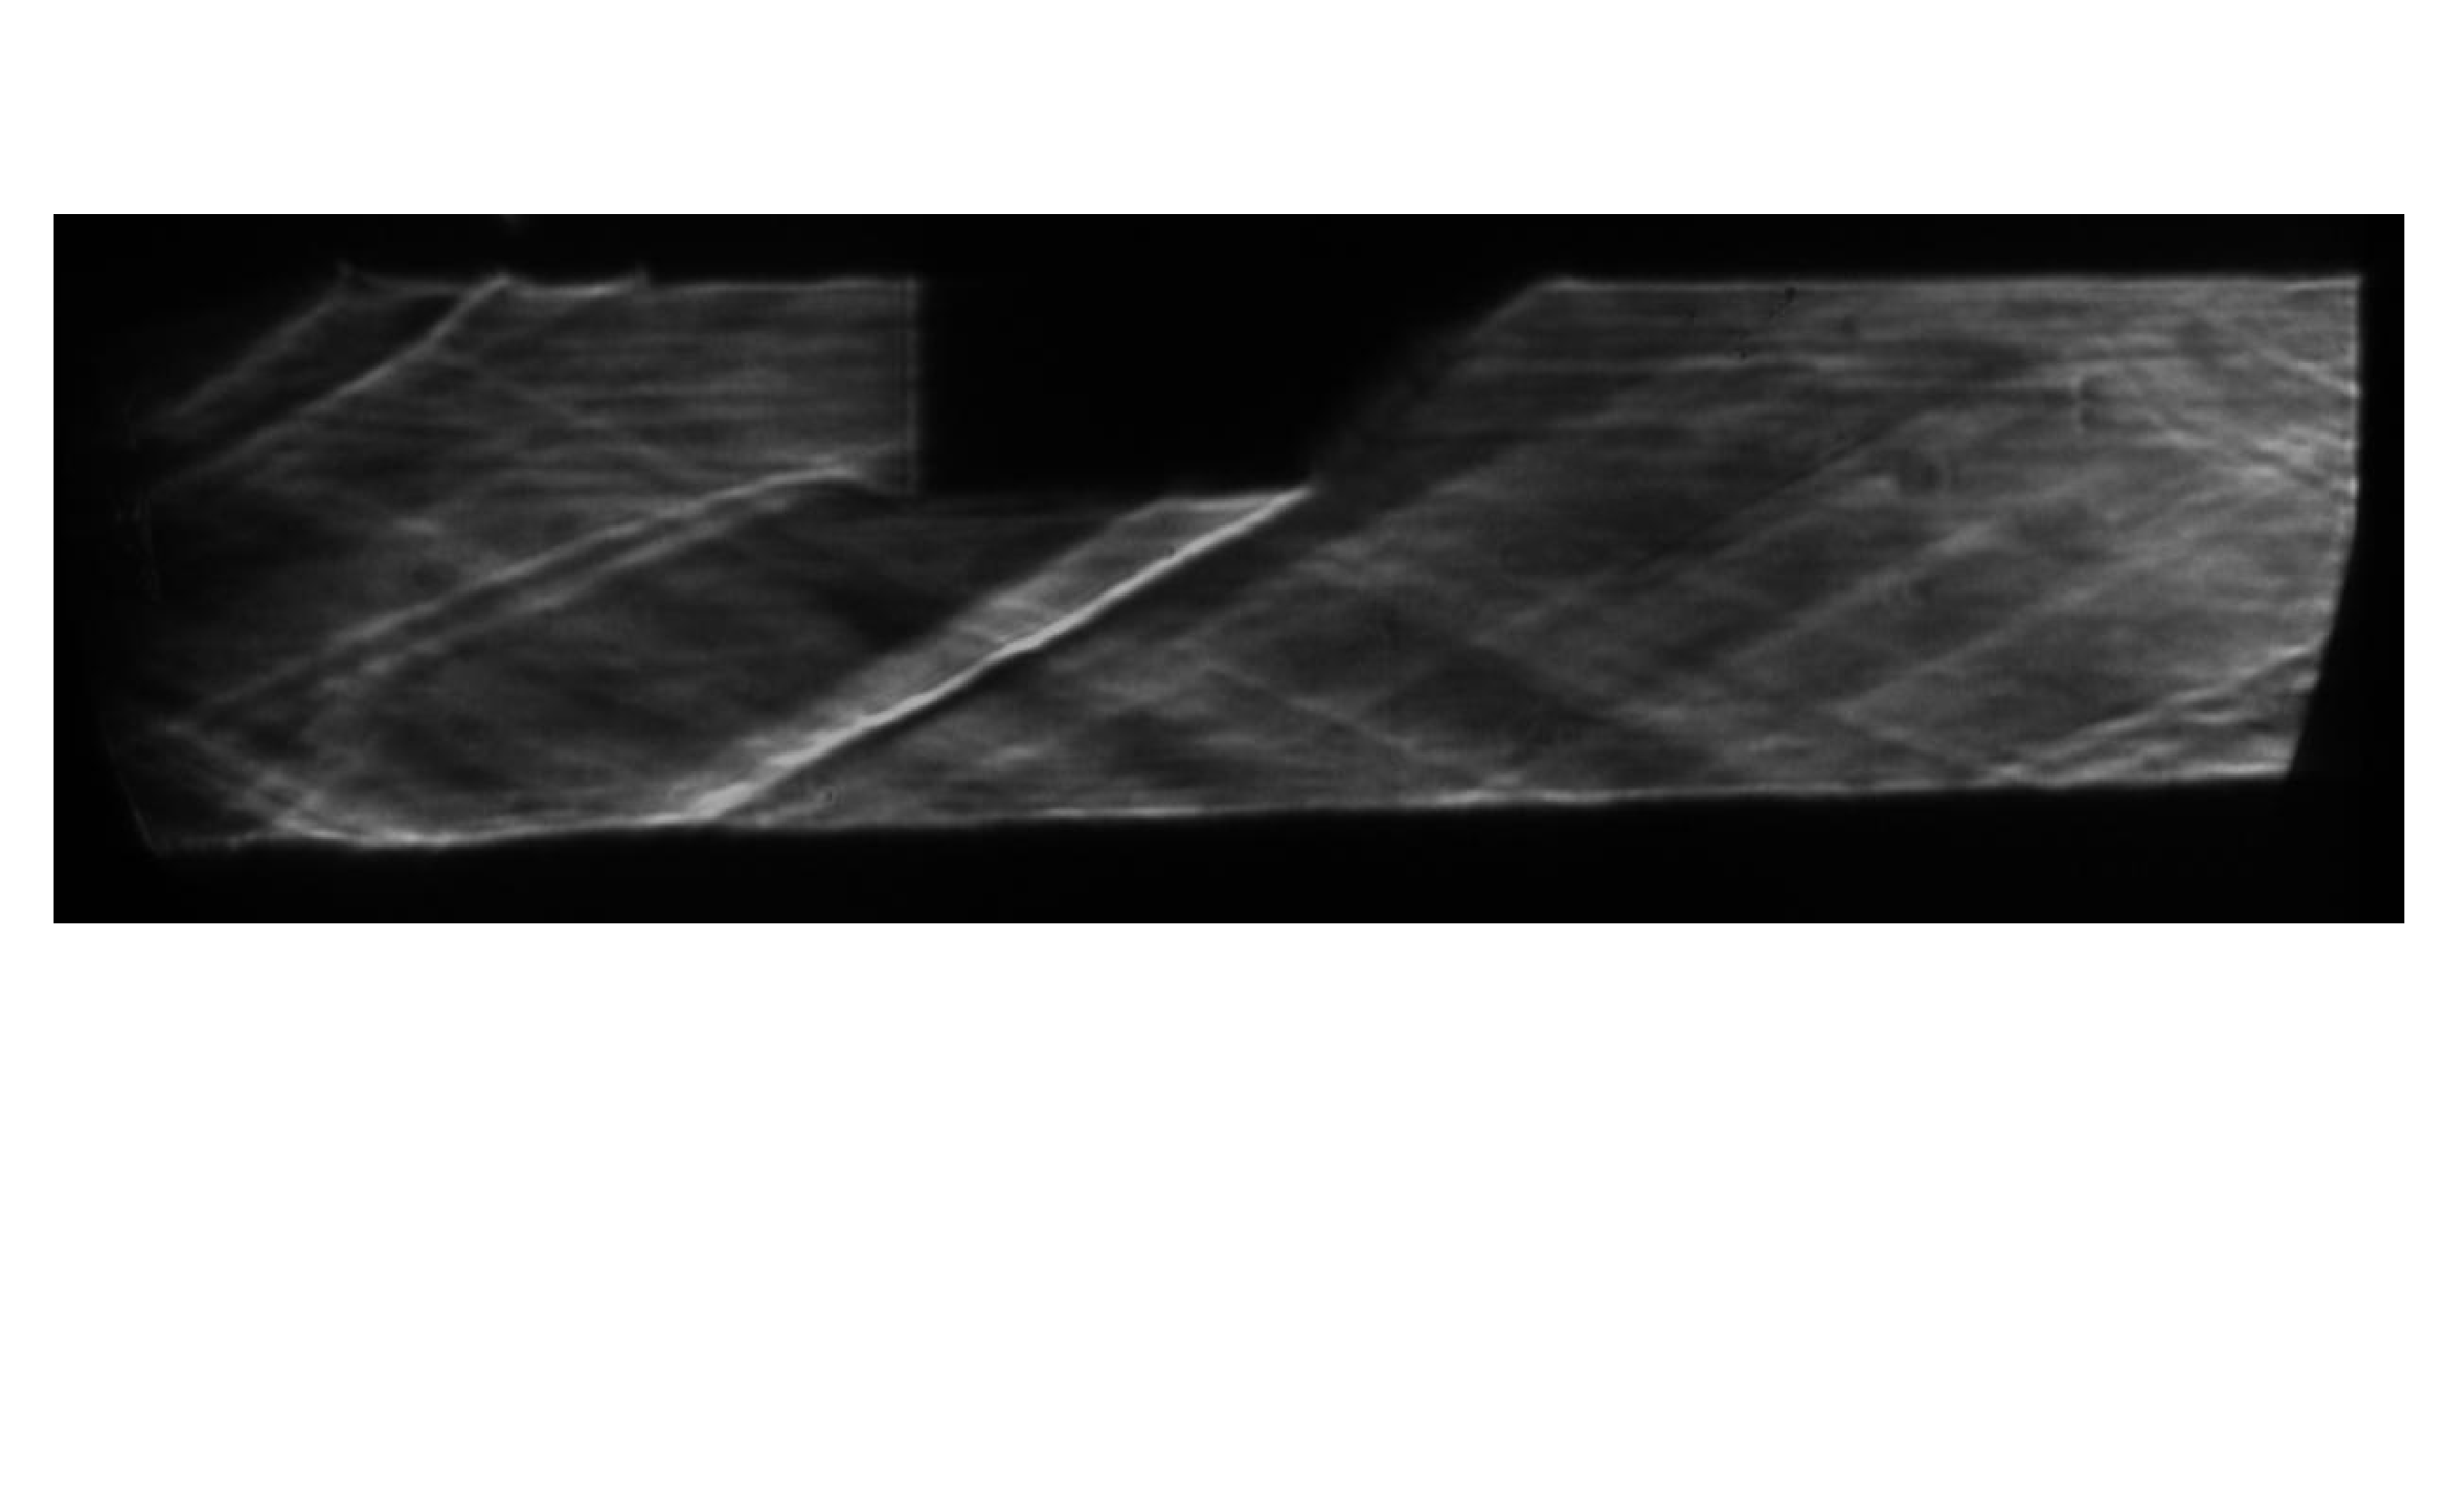
\includegraphics[width=0.95\textwidth]{WaveSchlieren3of4.pdf}}\\
(c)纹影法纵切3/4光线
\end{minipage}%
\begin{minipage}[b]{.5\textwidth}
\centering
\fbox{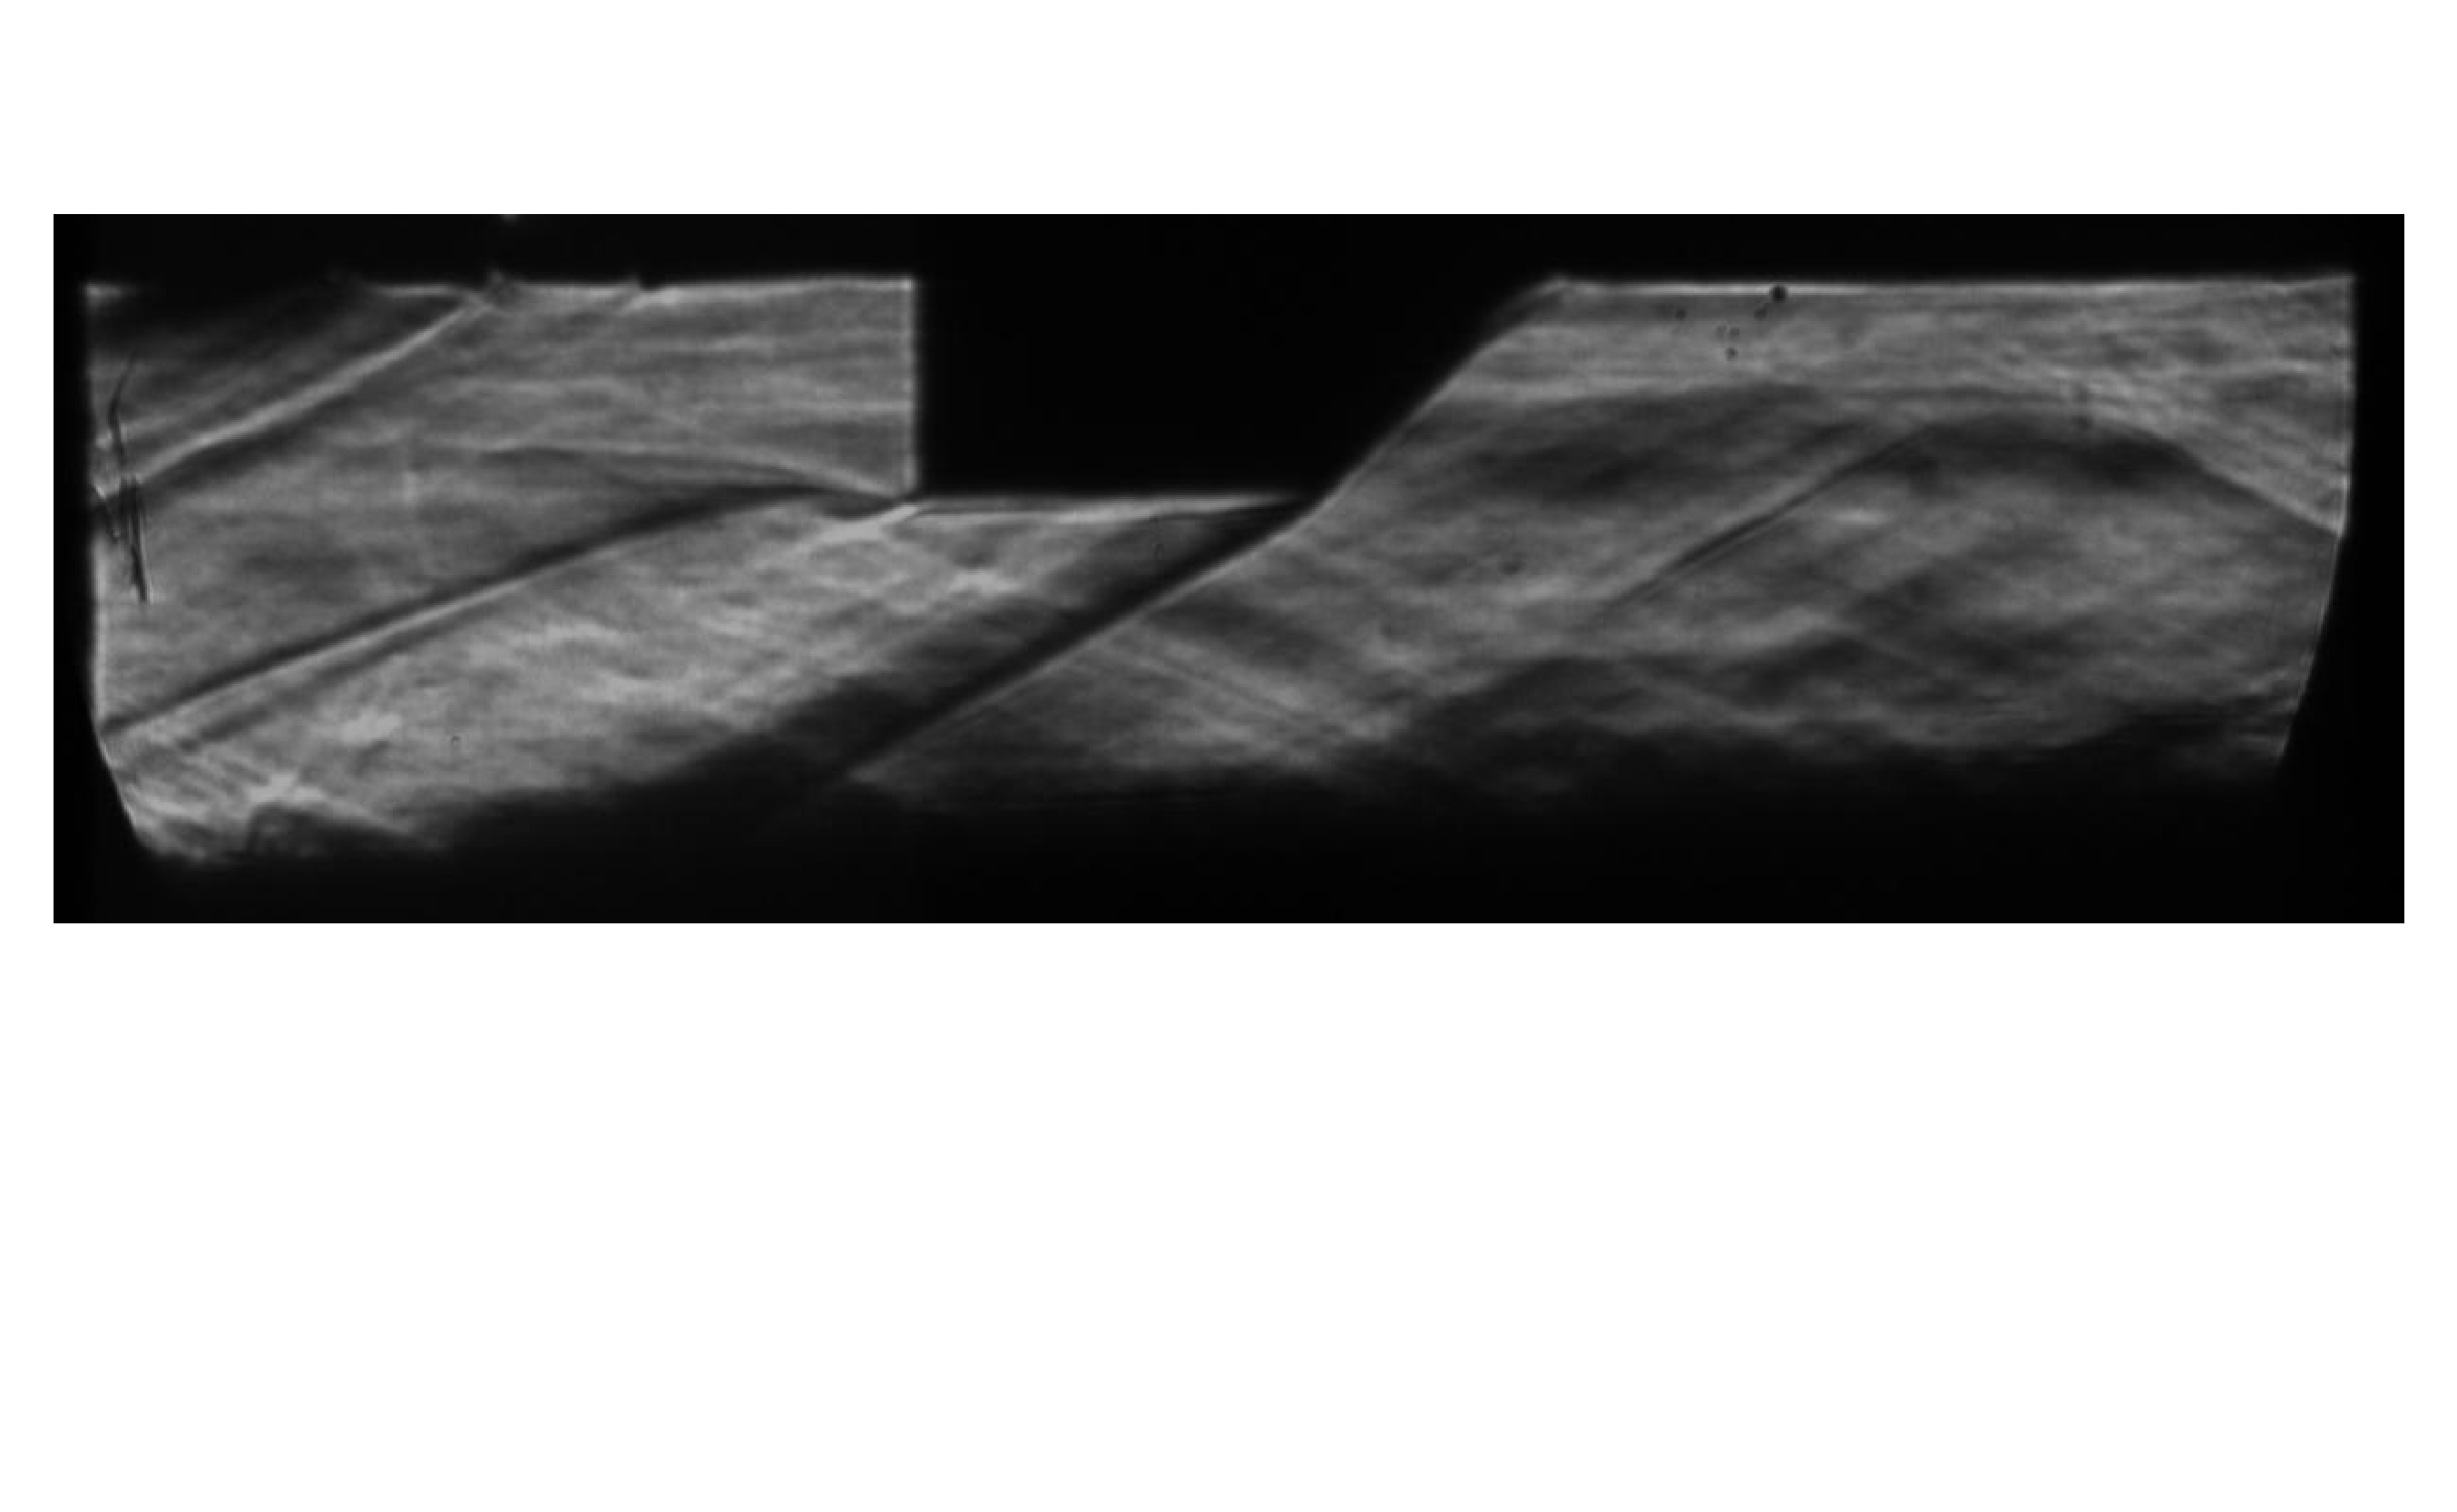
\includegraphics[width=0.95\textwidth]{WaveHSchlieren1of2.pdf}}\\
(d)纹影法横切1/2光线
\end{minipage}
\caption{\label{wave}四种情况下的激波图案}
\end{figure}



\subsection{结果分析}
图\ref{wave}中四个子图所显示流场信息大致相同, 仅在明暗上及细节处有差别, 下面取阴影法图单独分析. 将图\ref{wave}中的(a)图取出并标号得到图\ref{marker}.
\begin{figure}[!htb]
\centering
\fbox{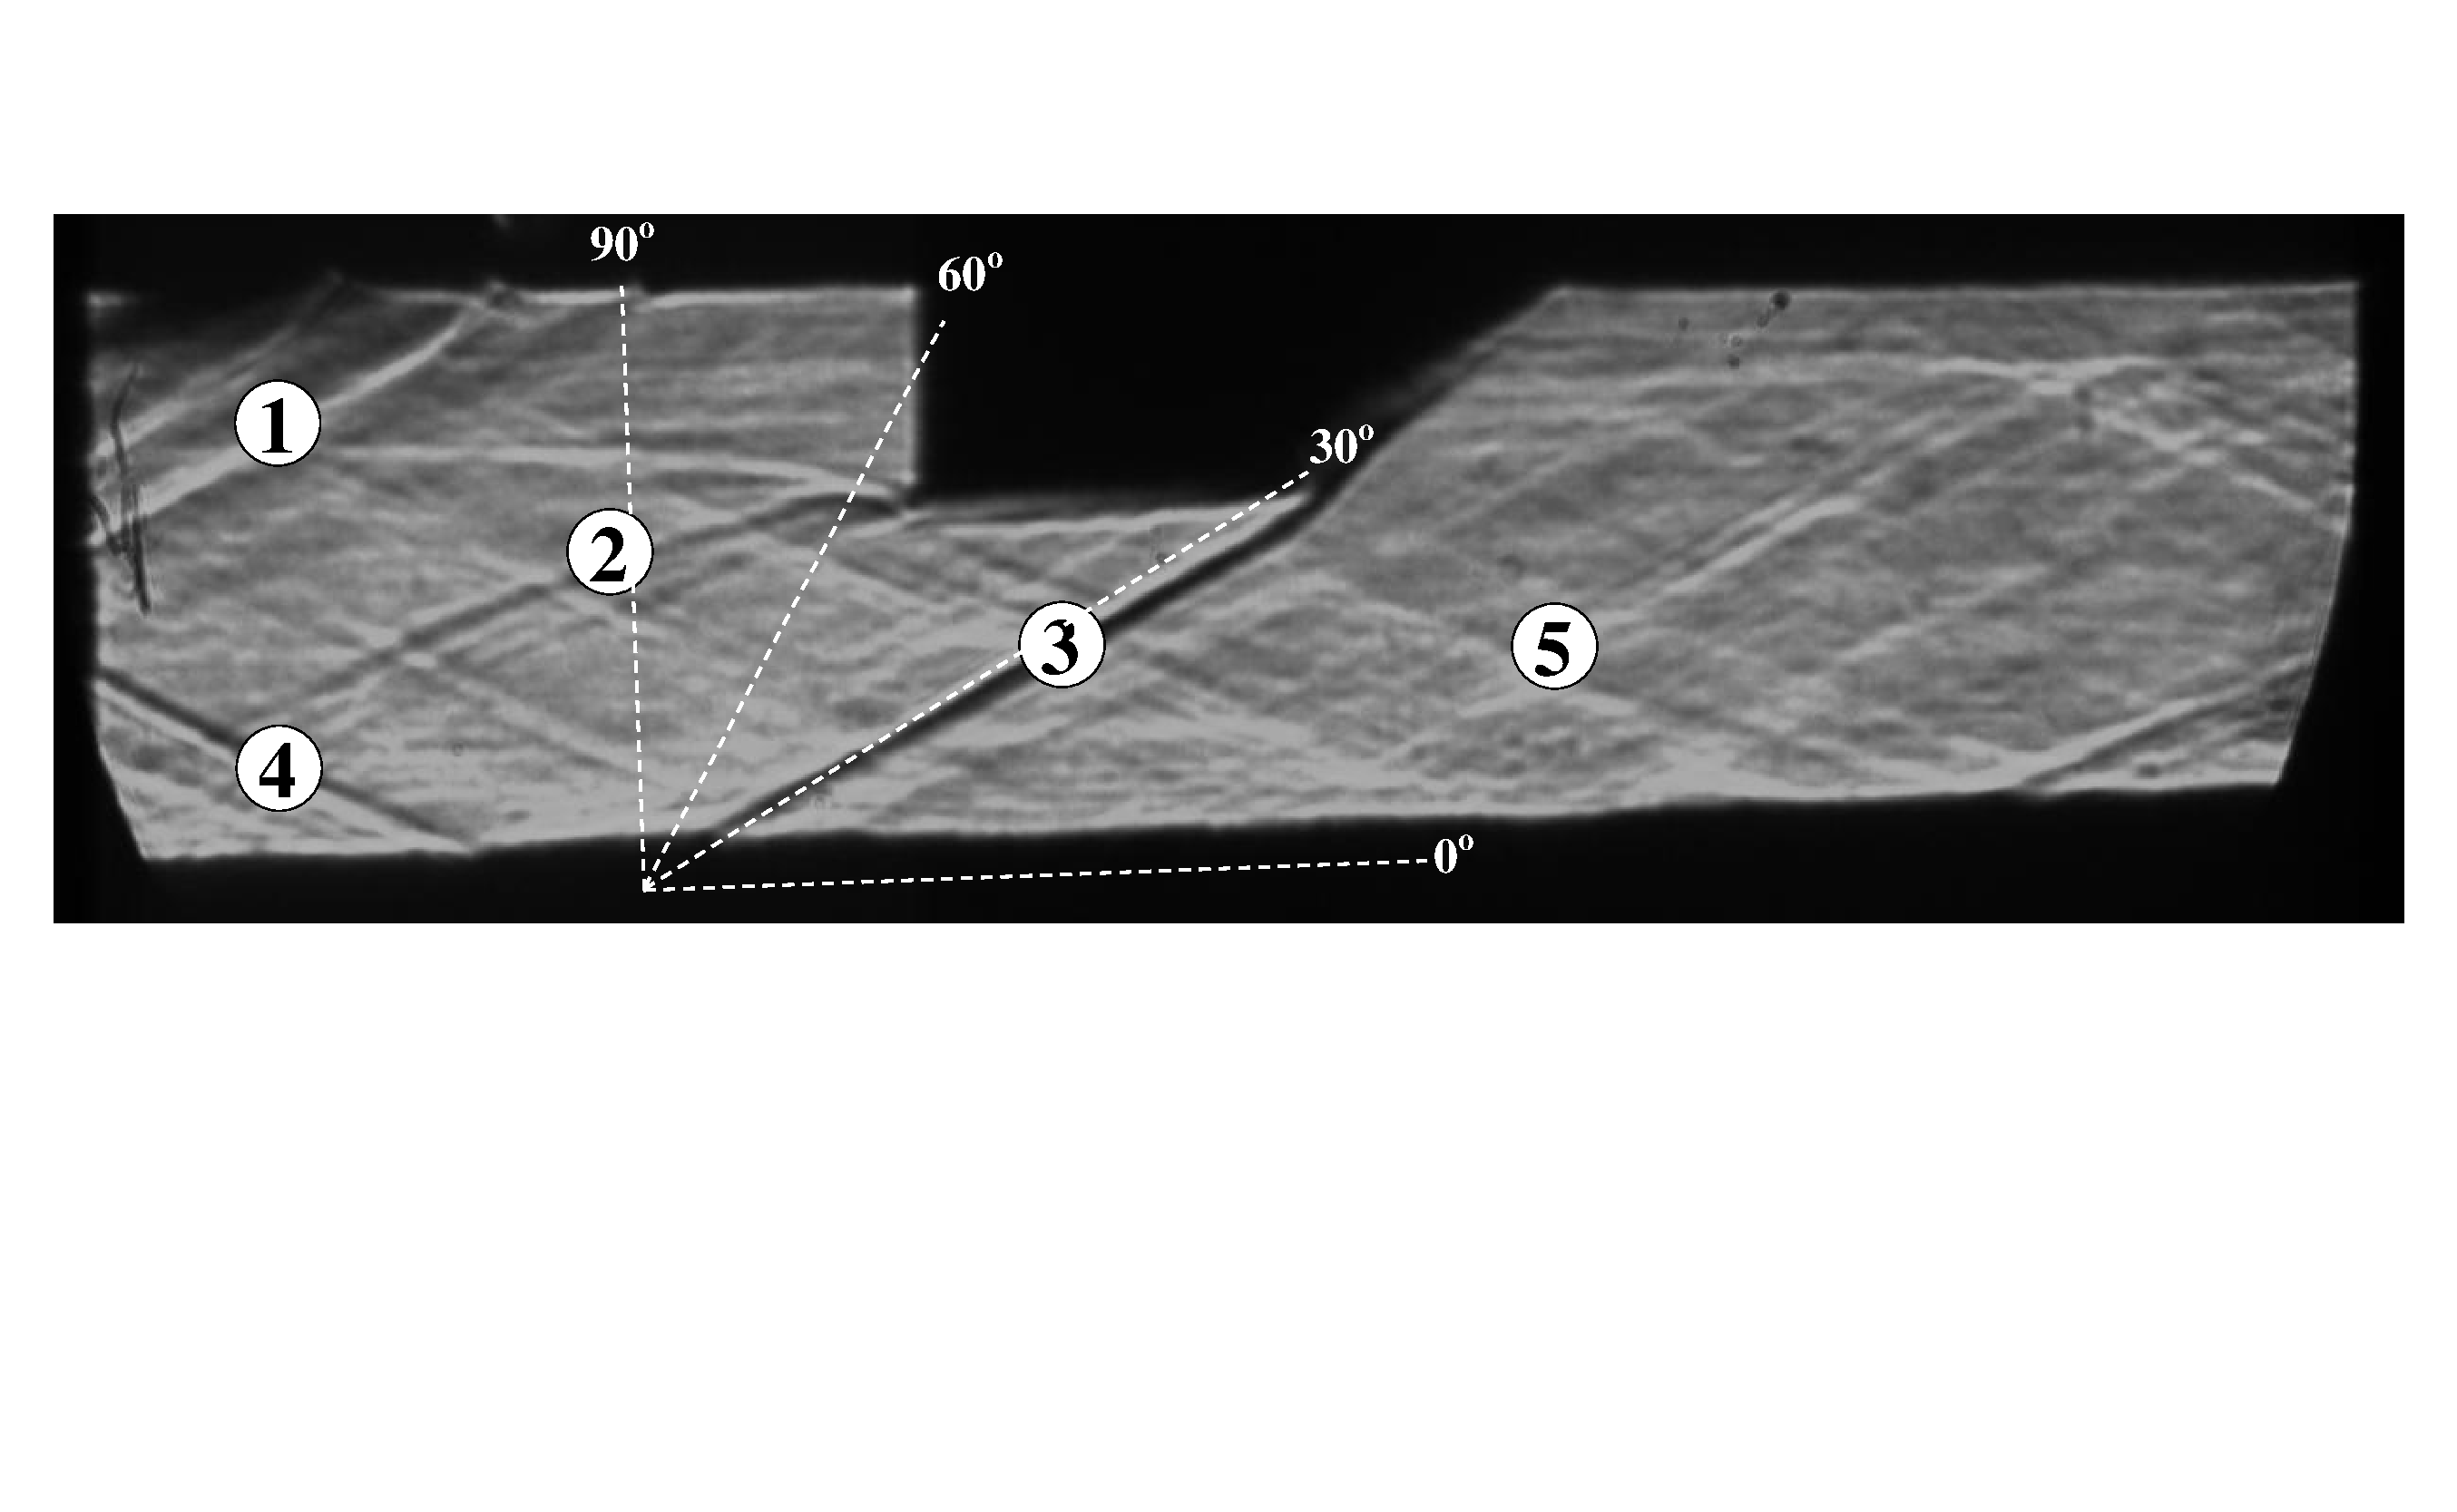
\includegraphics[width=0.97\textwidth]{WaveShadowMarker.pdf}}
\caption{\label{marker}阴影法测得的激波图案(带标号)}
\end{figure}
下面对图\ref{marker}所示流场中的5个标号位置出现的现象加以说明:
\begin{enumerate}
\item 由于燃烧室内流道内壁有突起造成干扰波.
\item 是膨胀波系.
\item 是一个激波.
\item 是3处的激波在壁面的反射波.
\item 类似的细小的纹路是前部的壁面扰动与其在风动内部反射的结果, 属于杂波, 可以不考虑.
\end{enumerate}
下面, 着重分析3处的激波. 3处显暗纹, 为一激波区域. 如图\ref{analysis}所示, $v_1$和 $v_2$分别是波前和波后的速度. 前后$v^t$不发生变化, 即$v_1^t = v_2^t$, 而$v^n$减小, 即$v_1^n>v_2^n$.
\begin{figure}[!htb]
\centering
\fbox{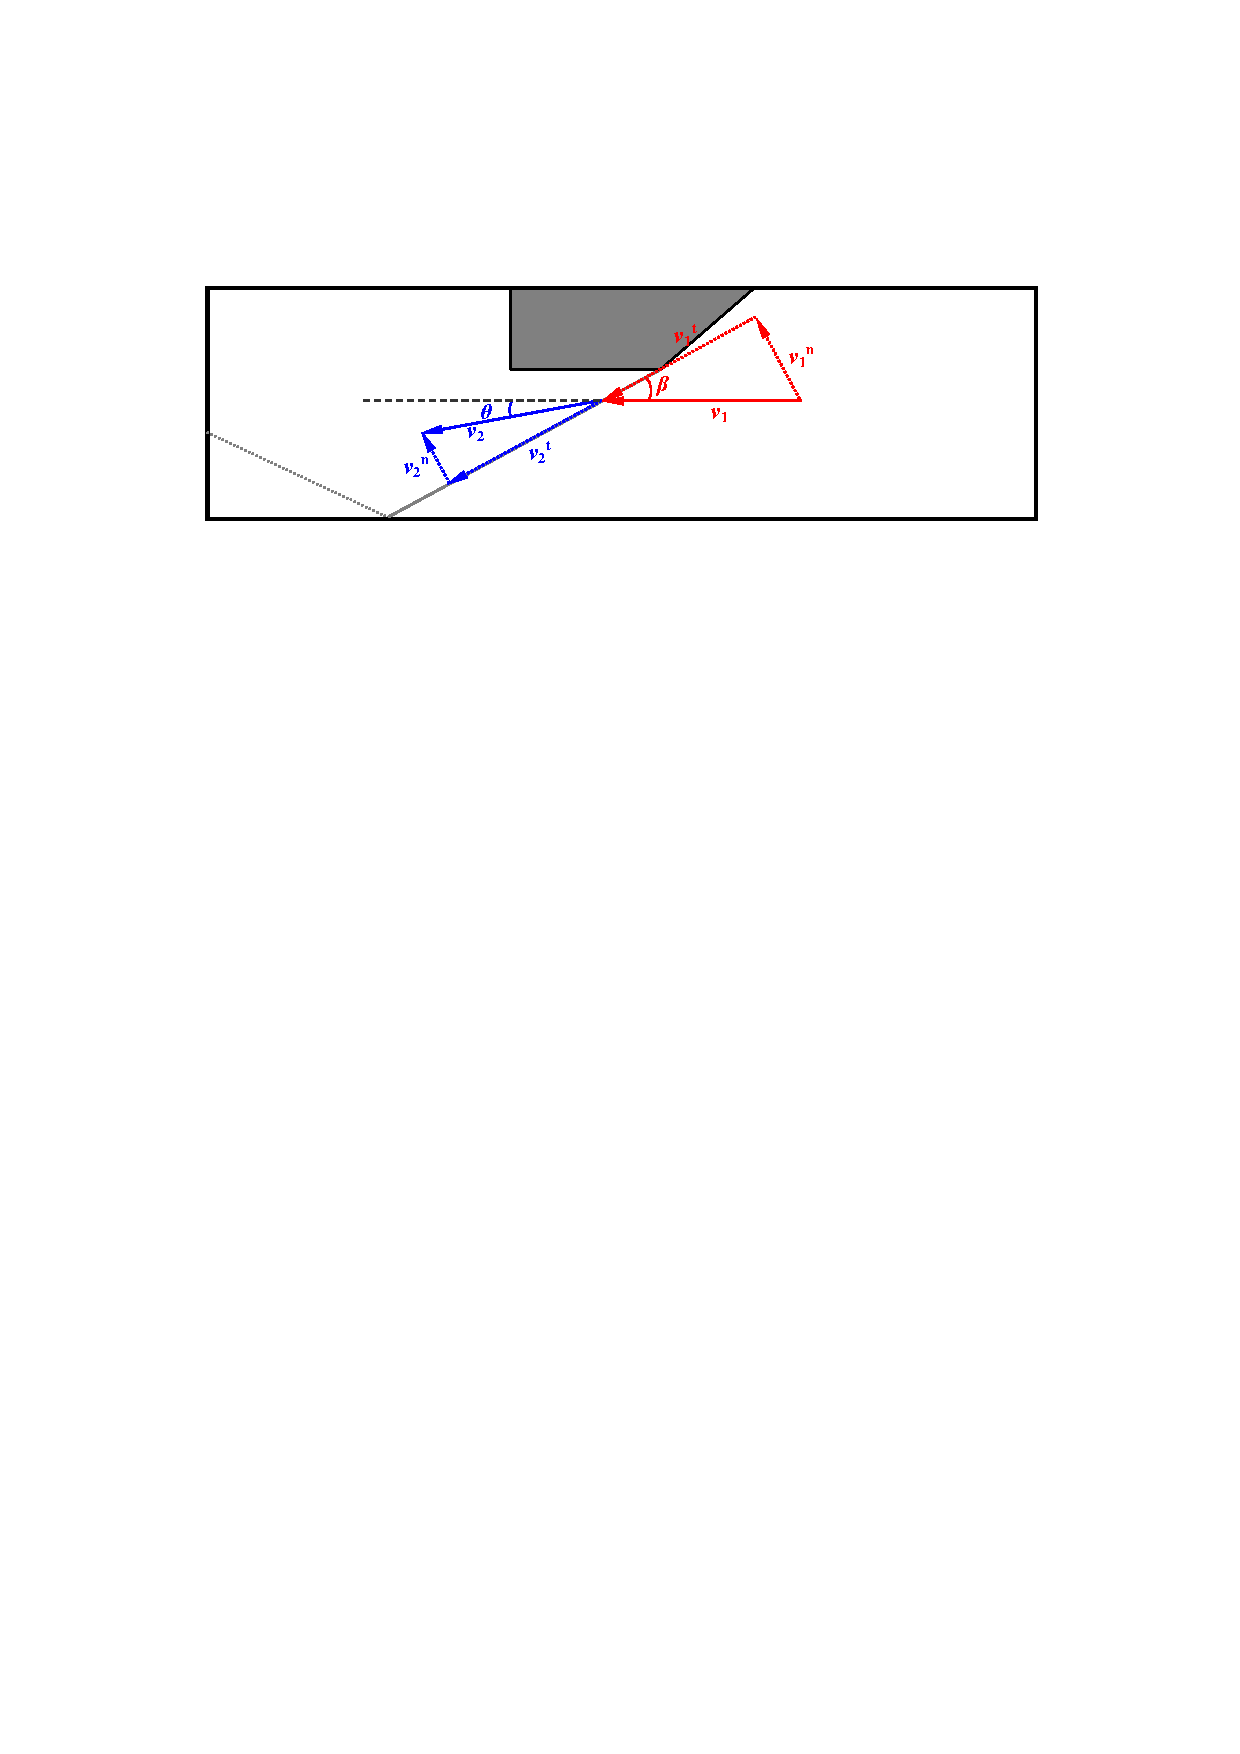
\includegraphics[width=0.97\textwidth]{analysis.pdf}}
\caption{\label{analysis}激波分析图}
\end{figure}
由图\ref{analysis}中的几何关系有
\[
\tan\beta = \frac{v_1^n}{v_1^t}, {~~}\tan(\beta-\theta)=\frac{v_2^n}{v_1^t}
\]
而$v_1^t = v_2^t$, 因此由上式可得
\[
\frac{\tan(\beta-\theta)}{\tan\beta} = \frac{v_2^n}{v_1^n} = \frac{\rho_1}{\rho_2} = \frac{2+(\gamma-1)M_1\sin^2\beta}{(\gamma+1)M_1\sin^2\beta}
\]
上式中$M_1$为波前马赫数, 化简可得
\[
\tan\theta = \frac{M_1^2\sin^2\beta-1}{M_1^2(\gamma+\cos 2\beta)+2}
\]
由于3处壁面影响, 波前波后的速度都应平行壁面, 即$\theta = 0$. 因此$\beta=\pi/2$或$\sin\beta=\frac{1}{M_1}$, 此处应为$\sin\beta=\frac{1}{M_1}$. 由图\ref{marker}可知$\beta\approx\pi/6$, 因此波前马赫数$M_1\approx2$.

\section{结论}
本实验应用光学方法清楚的程现激波流场, 并利用高速摄相机计算数据. 数据较为精确, 为流体力学的理论研究和数值模拟提供可靠的实验依据. 通过本实验测得的流场信息, 成功的返推出流场的马赫数, 这同时也证明实验的正确性. 另外, 通过本实验可知 阴影法只对密度的二阶导数灵敏, 适用于密度梯度变化显著的流场显示, 如激波等. 纹影法对密度梯度灵敏, 比阴影法有更多的细节分辨, 能显示连续变化的密度场. 纹影图有明暗相间的条纹, 显示的细节比较多, 而阴影图除了显示斜激波外, 流场其他地方基本一样.

实验中也有许多不足, 导致一定的误差. 如调制平行光时, 测量误差影响平行光的平行程度. 平行光图像放大率为1, 像与原物相当, 测量时选了两个参考物, 凹面镜和试验段的矩形框. 凹面镜的像是圆形光圈, 由于圆心位置不确定, 测量直径时难免有误差: 另外试验段的前后两块玻璃由于不是正对的, 有效长度应为正对长度, 测量时也会有误差, 导致平行光的平行程度不够. 另外, 试验段的玻璃不够光滑, 光透过玻璃后, 亮度和平行度都受到了影响, 质量变差, 也会影响了照片的清晰度.

流场的显示技术对流体力学的发展起到了重要的作用.  虽然阴影, 纹影等光学技术比较古典, 但目前仍大量服务于各种技术领域, 并由于结合激光得到一些新进展. 今后的科学发展需要流场显示技术提供更多, 更精密的流场数据和流谱图象, 从而
建立更为精确的物理模型.



\begin{thebibliography}{99}
\bibitem{0} 束继祖, 李华煌. 流场显示技术在流体力学中
的应用和展望. 力学进展, 1979(01): 002
\bibitem{1} Physical solutions of everyday problems in aquatic sciences.\\
 \textit{http://misclab.umeoce.maine.edu/boss/classes/SMS\_491\_2003/Week\_5.htm}.
\bibitem{1} 李桂春. 风洞试验光学测量方法. 国防工业出版社, 2008.
\bibitem{2}Werle, H. Annual Rev. of Fluid Mechanics, 5(1973), 361.
\end{thebibliography}

\end{document}
